\documentclass[notes,11pt, aspectratio=169]{beamer}

\usepackage{pgfpages}
% These slides also contain speaker notes. You can print just the slides,
% just the notes, or both, depending on the setting below. Comment out the want
% you want.
\setbeameroption{hide notes} % Only slide
%\setbeameroption{show only notes} % Only notes
%\setbeameroption{show notes on second screen=right} % Both

\usepackage{helvet}
\usepackage[default]{lato}
\usepackage{array}
\usepackage{tgbonum}

\usepackage{tikz}
\usepackage{verbatim}
\setbeamertemplate{note page}{\pagecolor{yellow!5}\insertnote}
\usetikzlibrary{positioning}
\usetikzlibrary{snakes}
\usetikzlibrary{calc}
\usetikzlibrary{arrows}
\usetikzlibrary{decorations.markings}
\usetikzlibrary{shapes.misc}
\usetikzlibrary{matrix,shapes,arrows,fit,tikzmark}
\usepackage{amsmath}
\usepackage{mathpazo}
\usepackage{hyperref}
\usepackage{lipsum}
\usepackage{multimedia}
\usepackage{graphicx}
\usepackage{multirow}
\usepackage{graphicx}
\usepackage{dcolumn}
\usepackage{bbm}
\newcolumntype{d}[0]{D{.}{.}{5}}

\usepackage{changepage}
\usepackage{appendixnumberbeamer}
\newcommand{\beginbackup}{
   \newcounter{framenumbervorappendix}
   \setcounter{framenumbervorappendix}{\value{framenumber}}
   \setbeamertemplate{footline}
   {
     \leavevmode%
     \hline
     box{%
       \begin{beamercolorbox}[wd=\paperwidth,ht=2.25ex,dp=1ex,right]{footlinecolor}%
%         \insertframenumber  \hspace*{2ex} 
       \end{beamercolorbox}}%
     \vskip0pt%
   }
 }
\newcommand{\backupend}{
   \addtocounter{framenumbervorappendix}{-\value{framenumber}}
   \addtocounter{framenumber}{\value{framenumbervorappendix}} 
}


\usepackage{graphicx}
\usepackage[space]{grffile}
\usepackage{booktabs}
\newcommand\independent{\protect\mathpalette{\protect\independenT}{\perp}}
\def\independenT#1#2{\mathrel{\rlap{$#1#2$}\mkern2mu{#1#2}}}
\DeclareMathOperator{\Supp}{Supp}

% These are my colors -- there are many like them, but these ones are mine.
\definecolor{blue}{RGB}{0,114,178}
\definecolor{red}{RGB}{213,94,0}
\definecolor{yellow}{RGB}{240,228,66}
\definecolor{green}{RGB}{0,158,115}

\hypersetup{
  colorlinks=false,
  linkbordercolor = {white},
  linkcolor = {blue}
}


%% I use a beige off white for my background
\definecolor{MyBackground}{RGB}{255,253,218}

%% Uncomment this if you want to change the background color to something else
%\setbeamercolor{background canvas}{bg=MyBackground}

%% Change the bg color to adjust your transition slide background color!
\newenvironment{transitionframe}{
  \setbeamercolor{background canvas}{bg=yellow}
  \begin{frame}}{
    \end{frame}
}

\setbeamercolor{frametitle}{fg=blue}
\setbeamercolor{title}{fg=black}
\setbeamertemplate{footline}[frame number]
\setbeamertemplate{navigation symbols}{} 
\setbeamertemplate{itemize items}{-}
\setbeamercolor{itemize item}{fg=blue}
\setbeamercolor{itemize subitem}{fg=blue}
\setbeamercolor{enumerate item}{fg=blue}
\setbeamercolor{enumerate subitem}{fg=blue}
\setbeamercolor{button}{bg=MyBackground,fg=blue,}



% If you like road maps, rather than having clutter at the top, have a roadmap show up at the end of each section 
% (and after your introduction)
% Uncomment this is if you want the roadmap!
% \AtBeginSection[]
% {
%    \begin{frame}
%        \frametitle{Roadmap of Talk}
%        \tableofcontents[currentsection]
%    \end{frame}
% }
\setbeamercolor{section in toc}{fg=blue}
\setbeamercolor{subsection in toc}{fg=red}
\setbeamersize{text margin left=1em,text margin right=1em} 

\newenvironment{wideitemize}{\itemize\addtolength{\itemsep}{10pt}}{\enditemize}

\usepackage{environ}
\NewEnviron{videoframe}[1]{
  \begin{frame}
    \vspace{-8pt}
    \begin{columns}[onlytextwidth, T] % align columns
      \begin{column}{.70\textwidth}
        \begin{minipage}[t][\textheight][t]
          {\dimexpr\textwidth}
          \vspace{8pt}
          \hspace{4pt} {\Large \sc \textcolor{blue}{#1}}
          \vspace{8pt}
          
          \BODY
        \end{minipage}
      \end{column}%
      \hfill%
      \begin{column}{.38\textwidth}
        \colorbox{green!20}{\begin{minipage}[t][1.2\textheight][t]
            {\dimexpr\textwidth}
            Face goes here
          \end{minipage}}
      \end{column}%
    \end{columns}
  \end{frame}
}

\title[]{\textcolor{blue}{Linear Regression III: Quantile Estimation}}
\author[PGP]{}
\institute[FRBNY]{\small{Paul Goldsmith-Pinkham}}
\date{\today}


\begin{document}

%%% TIKZ STUFF
\tikzset{   
        every picture/.style={remember picture,baseline},
        every node/.style={anchor=base,align=center,outer sep=1.5pt},
        every path/.style={thick},
        }
\newcommand\marktopleft[1]{%
    \tikz[overlay,remember picture] 
        \node (marker-#1-a) at (-.3em,.3em) {};%
}
\newcommand\markbottomright[2]{%
    \tikz[overlay,remember picture] 
        \node (marker-#1-b) at (0em,0em) {};%
}
\tikzstyle{every picture}+=[remember picture] 
\tikzstyle{mybox} =[draw=black, very thick, rectangle, inner sep=10pt, inner ysep=20pt]
\tikzstyle{fancytitle} =[draw=black,fill=red, text=white]
%%%% END TIKZ STUFF

% Title Slide
\begin{frame}
\maketitle

\end{frame}


\begin{frame}{A brief refresher on OLS (and GMM)}
  \begin{columns}[T] % align columns
\begin{column}{.8\textwidth}
  \begin{wideitemize}
  \item Recall that OLS is the ``least-squares'' method -- it can be
    defined as the method that minimizes the sum of squared ``errors''
    \begin{itemize}
    \item These errors are the residuals from say, our linear model:
      $$E(y_{i}|x_{i}) = x_{i}\beta, \qquad \hat{\beta}_{ls} = \arg\min_{\beta} \sum_{i} (y_{i} - x_{i}\beta)^{2} = \arg\min_{\beta} (\mathbf{Y} - \mathbf{X}\beta)'(\mathbf{Y} - \mathbf{X}\beta) $$
    \item No surprise -- the least squares method is finding the ``least'' of the squares. In particular, we can use calculus to get our analytic solution, since we're trying to minimize an objective function:
$$ -\mathbf{X}'(\mathbf{Y} - \mathbf{X}\hat{\beta})  = 0 \qquad  -\mathbf{X}'\mathbf{Y}  + \mathbf{X}'\mathbf{X}\hat{\beta}  = 0 \qquad  \hat{\beta}  = (\mathbf{X}'\mathbf{X})^{-1}\mathbf{X}'\mathbf{Y} $$
\end{itemize}
\item The least squares does a lot of work for us by creating a nice
  objective function
  \begin{itemize}
  \item Beyond that, what does a quadratic obj. function do?
  \end{itemize}
  \end{wideitemize}
  \end{column}%
  \hfill%
  \begin{column}{.5\textwidth}
  \end{column}
\end{columns}
\end{frame}

\begin{frame}{A brief refresher on OLS (and GMM)}
  \begin{columns}[T] % align columns
\begin{column}{.8\textwidth}
  \begin{wideitemize}
  \item Key features of OLS:
    \begin{itemize}
    \item Squared loss function leads to heavily penalization from big outliers
    \item Local approximation to the conditional expectation function
      -- OLS finds the closest linear fit to the CEF
    \item In context of treatment effects, gives us approximation to the
      ATE
    \end{itemize}
  \item Most important feature of OLS for today: it characterizes
    features of the mean of our outcome variable, conditional on
    covariates (e.g. treatments)
    \begin{itemize}
    \item What if we care about other things?
    \item What are some properties of means that are problematic?
      \begin{itemize}
      \item Very sensitive to outliers!
      \end{itemize}
    \end{itemize}
  \end{wideitemize}
  \end{column}%
  \hfill%
  \begin{column}{.5\textwidth}
  \end{column}
\end{columns}
\end{frame}

\begin{frame}{Quantiles - some definitions}
  \begin{columns}[T] % align columns
\begin{column}{.7\textwidth}
  \begin{wideitemize}
  \item First, recall that for any r.v. $X$ we can define its CDF and inverse CDF:
    $$F(x) = Pr(X \leq x), \qquad F^{-1}(\tau) = \inf\{x : F(x) \geq \tau\}$$
    \begin{itemize}
    \vspace{-15pt}      
    \item The infimum deals with ties
    \item $\tau = 0.5$ is the median!
    \end{itemize}
  \item Consider now the following loss function:
    $$ \rho_{\tau}(u) = u \tau 1(u > 0) + u(\tau-1) 1(u <0) = u(\tau - 1(u<0))$$
    \vspace{-15pt}
    \begin{itemize}
    \item $\tau = 0.5 \longrightarrow \rho_{\tau}(u) = 0.5|u|$
    \end{itemize}
  \item We can talk about expected loss (a la  OLS):
    $$ E(\rho_\tau(X - \hat{\mu})) = \tau \int_{\hat{\mu}}^{\infty} (x - \hat{\mu}) dF(x) + (1-\tau) \int^{\hat{\mu}}_{-\infty} (x - \hat{\mu}) dF(x)$$
  \end{wideitemize}
  \end{column}%
  \hfill%
  \begin{column}{.3\textwidth}
    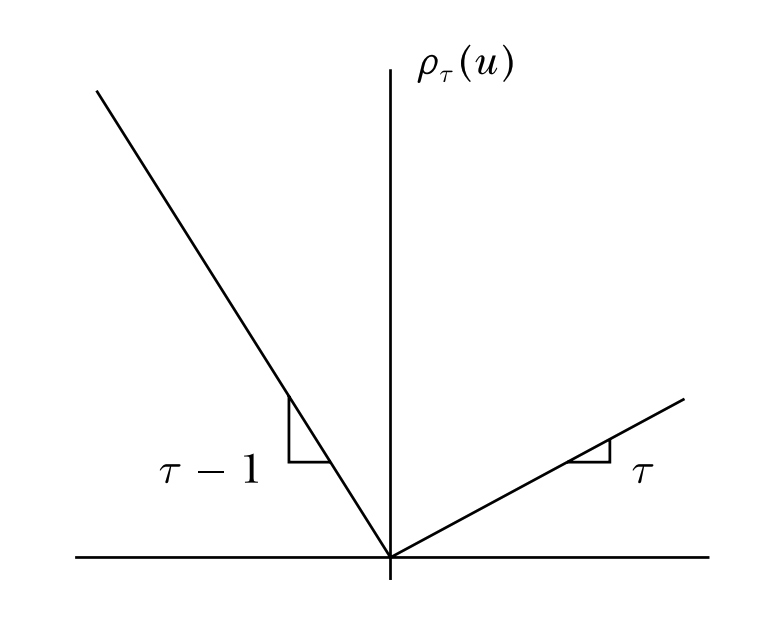
\includegraphics[width=\linewidth]{check_fn.png}
  \end{column}
\end{columns}
\end{frame}


\begin{frame}{Quantiles as solutions}
  \begin{columns}[T] % align columns
\begin{column}{.9\textwidth}
  \begin{align*}
    E(\rho_\tau(X - \hat{\mu})) &= \tau \int_{\hat{\mu}}^{\infty} (x - \hat{\mu}) dF(x) + (1-\tau) \int^{\hat{\mu}}_{-\infty} (x - \hat{\mu}) dF(x)\\
\rightarrow   \hat{\mu} &= F^{-1}(\tau) 
    \end{align*}
    \begin{wideitemize}
    \item This problem naturally lends itself to generalization. Let $Q_{\tau}(Y |X ) \equiv \inf\{y : F_{Y}(y | X)\geq \tau\}$ be the \emph{conditional quantile function}, analogous to the conditional expectation function
    \item This function minimizes the $\rho_{\tau}$ distance between some function of $X$ and $Y$:
      \begin{equation*}
        Q_{\tau}(Y | X) = \arg\min_{q(X)} E(\rho_{\tau}(Y - q(X)))
      \end{equation*}
    \item Just as we denoted approximated the conditional expectation
      function with a linear model, we can approximate the
      $Q_{\tau}(Y|X)$ with a linear model!
    \end{wideitemize}
  \end{column}%
  \hfill%
  \begin{column}{.3\textwidth}
  \end{column}
\end{columns}
\end{frame}

\begin{frame}{Quantiles as solutions}
  \begin{columns}[T] % align columns
\begin{column}{.9\textwidth}
    \begin{wideitemize}
    \item Consider now our linear model minimizer:
      \begin{equation*}
        \beta(\tau) \equiv \arg\min_{\beta} E(\rho_{\tau}(Y - X'\beta))
      \end{equation*}
    \item This is the best linear predictor under the $\rho$ loss function
      \begin{itemize}
      \item But how does it map to the true $Q_{\tau}(Y|X)$?
      \end{itemize}
    \item Key result from Angrist et al. (2006): this linear model is
      the weighted least squares approximation to the unknown CQF
      $$ \beta(\tau)  = \arg\min_{\beta}E\left[w_{\tau}(X, \beta) \Delta^{2}_{\tau}(X, \beta)\right], \qquad \Delta_{\tau}(X, \beta) = X'\beta - Q_{\tau}(Y|X),$$
      where the $w_{\tau}$ are \emph{importance} weights, and average
      over the difference between the true CQF and the linear
      approximation.
    \end{wideitemize}
  \end{column}%
  \hfill%
  \begin{column}{.3\textwidth}
  \end{column}
\end{columns}
\end{frame}


\begin{frame}{How is it solved?}
  \begin{wideitemize}
  \item Unlike OLS, there is no direct analytic solution for
    $\beta(\tau)$
    \begin{itemize}
    \item This implies that the problem needs to be solved numerically
    \end{itemize}
  \item Key insight: you can redefine the minimization problem of
    $$\hat{\beta}(\tau) = \arg\min_{\beta} \sum_{i=1}^{n} \rho_{\tau}(Y_{i} - X\beta)$$
    as a linear programming problem.
  \item We're not going to get into the details of this -- others have suffered for us
    \begin{itemize}
    \item See Chapter 6 of Koenker (2005)  or appendix of Koenker and Bassett
    (1978)
    \end{itemize}
  \end{wideitemize}
\end{frame}

\begin{frame}{Variance properties}
  \begin{wideitemize}
  \item Let's walk through thinking about the variance of a quantile. Let $\xi_{\tau} = F^{-1}(\tau)$, with density $f(\xi)$
    \begin{itemize}
    \item E.g. this is a quantile estimate
    \item How can we talk about its limiting properties?
    \end{itemize}
  \item Key trick: as we move around our estimate of $\xi_{\tau}$, we can think about the contribution that this has to our objective function (e.g. the gradient):
    $$g_{n}(\xi) = n^{-1}\sum_{i}1(Y_{i} < \xi) - \tau)$$
  \item As a result, you can think about the variability in our
    estimate coming from a series of coinflips on whether the data
    point is above or below the quantile estimate
    \begin{itemize}
    \item Convergence of the estimate is implied by the convergence
      of the empirical CDF to the true CDF
    \item Normality is a side benefit, and under iid data:
      $$ \sqrt{n}(\hat{\xi}_{\tau} - \xi_{\tau}) \rightarrow \mathcal{N}(0, \tau(1-\tau)f^{-2}(\xi_{\tau}))$$
    \end{itemize}
  \end{wideitemize}
\end{frame}


\begin{frame}{Variance properties}
  \begin{wideitemize}
  \item The non-i.i.d. error form of the limiting distribution for $\hat{\beta}(\tau)$ is familiar:
    \begin{align*}
    \sqrt{n}(\hat{\beta}(\tau) - \beta(\tau)) &\rightarrow \mathcal{N}(0, \tau(1-\tau)H^{-1}_{n}J_{n}H_{n}^{-1}\\
    J_{n}(\tau) &= n^{-1}\sum_{i}x_{i}'x_{i}\\
    H_{n}(\tau) &= n^{-1}\sum_{i}x_{i}'x_{i}f_{i}(\xi_{i}(\tau))
    \end{align*}
  \item The asymptotic variance of the estimator relies on knowledge of the density function
  \item That makes it harder (and slower!) to compute
  \item $\tau(1-\tau)$ is smaller in the tails, but $f_{i}$ is poorly
    estimated there, which tends to dominate.
  \end{wideitemize}
\end{frame}

\begin{frame}{Properties of Quantile Regressions (and sometimes OLS)}
  Equivariance (Koenker and Basset (1978)
  Consider a linear model $y = x\beta + epsilon$
  \begin{enumerate}
  \item Scale equivariance:
    \begin{itemize}
    \item scaling $y$ by some constant $a$ implies that $\hat{\beta} \rightarrow a\hat{\beta}$
    \end{itemize}
  \item Shift equivariance
    \begin{itemize}
    \item adding to $y$ some amount $X\gamma$ implies that $\hat{\beta} \rightarrow \hat{\beta} + X\gamma$
    \end{itemize}
  \item equivariance to reparametrization of design
    \begin{itemize}
    \item Linear combinations of regressors leads to linear combinations of coefficients
    \end{itemize}
  \item \emph{equivariance to monotone transformations}
    \begin{itemize}
      \item Let $h(\cdot)$ be monotone function
      \item $Q_{h(Y)}(\tau) = h(Q_{Y}(\tau))$
      \item E.g. the median of log(Y) is the log of the median of $Y$!
      \item Something OLS does \emph{not} have
      \end{itemize}
    \item The influence function of quantile regression is \emph{bounded} with respect to $y$
      \begin{itemize}
      \item This is not the case for OLS (outliers can have unlimited influence)
      \end{itemize}
  \end{enumerate}
\end{frame}

\begin{frame}{Practically, why are these properties useful?}
  \begin{wideitemize}
  \item Skewed variables-- no more worrying about logs or outliers in the outcome variable
  \item Censoring -- in many datasets, our outcome variables are top-coded or bottom-coded
    \begin{itemize}
    \item Note that given the influence function results, this is not
      a problem -- we can still identify (some) of the quantile
      functions
    \end{itemize}
  \item Let's look at an example
  \end{wideitemize}
\end{frame}

\begin{frame}{Quantile regression}
  \begin{columns}[T] % align columns
\begin{column}{.3\textwidth}
  \begin{wideitemize}
    \item Education + Income  gradient
  \item Clear heteroskedasticity
    \end{wideitemize}
  \end{column}%
  \hfill%
  \begin{column}{.7\textwidth}
    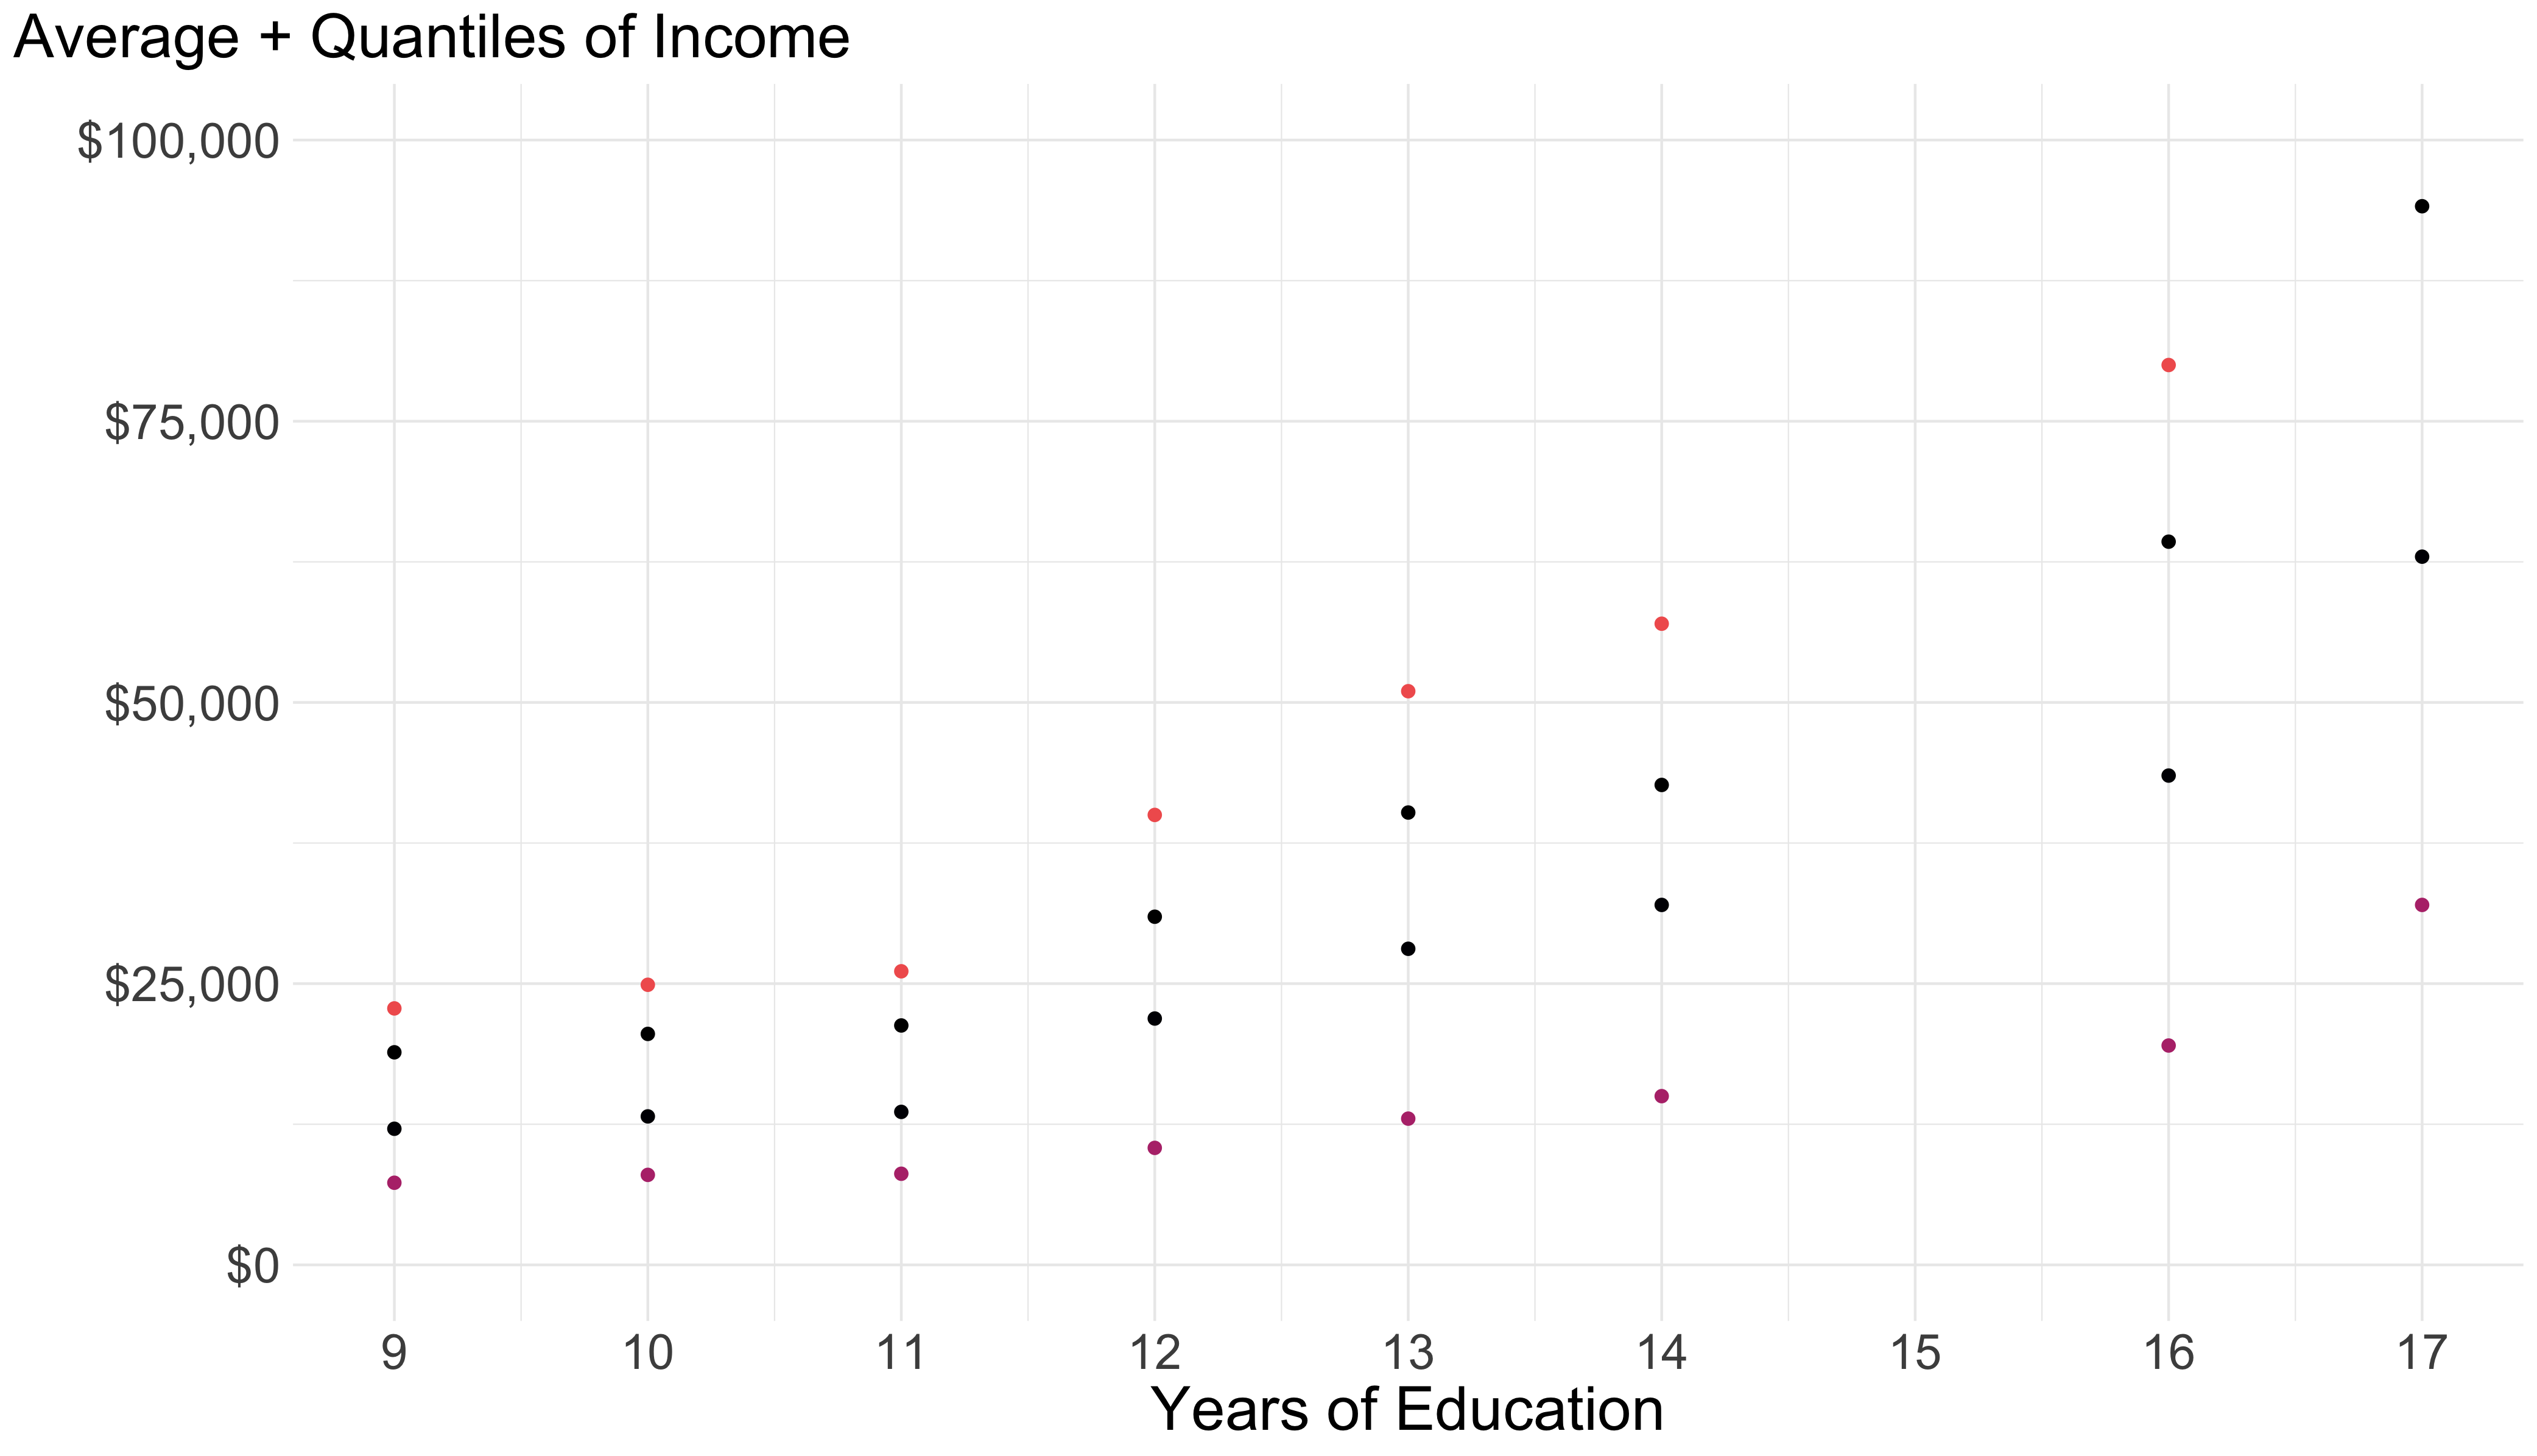
\includegraphics[width=\linewidth]{avg_income_education_mean.png}
  \end{column}
\end{columns}
\end{frame}

\begin{frame}{Quantile regression}
  \begin{columns}[T] % align columns
    \begin{column}{.3\textwidth}
  \begin{wideitemize}
    \item Education + Income  gradient
    \item Clear heteroskedasticity
    \item Very wide variance, especially at high education
  \end{wideitemize}
  \end{column}%
  \hfill%
  \begin{column}{.7\textwidth}
    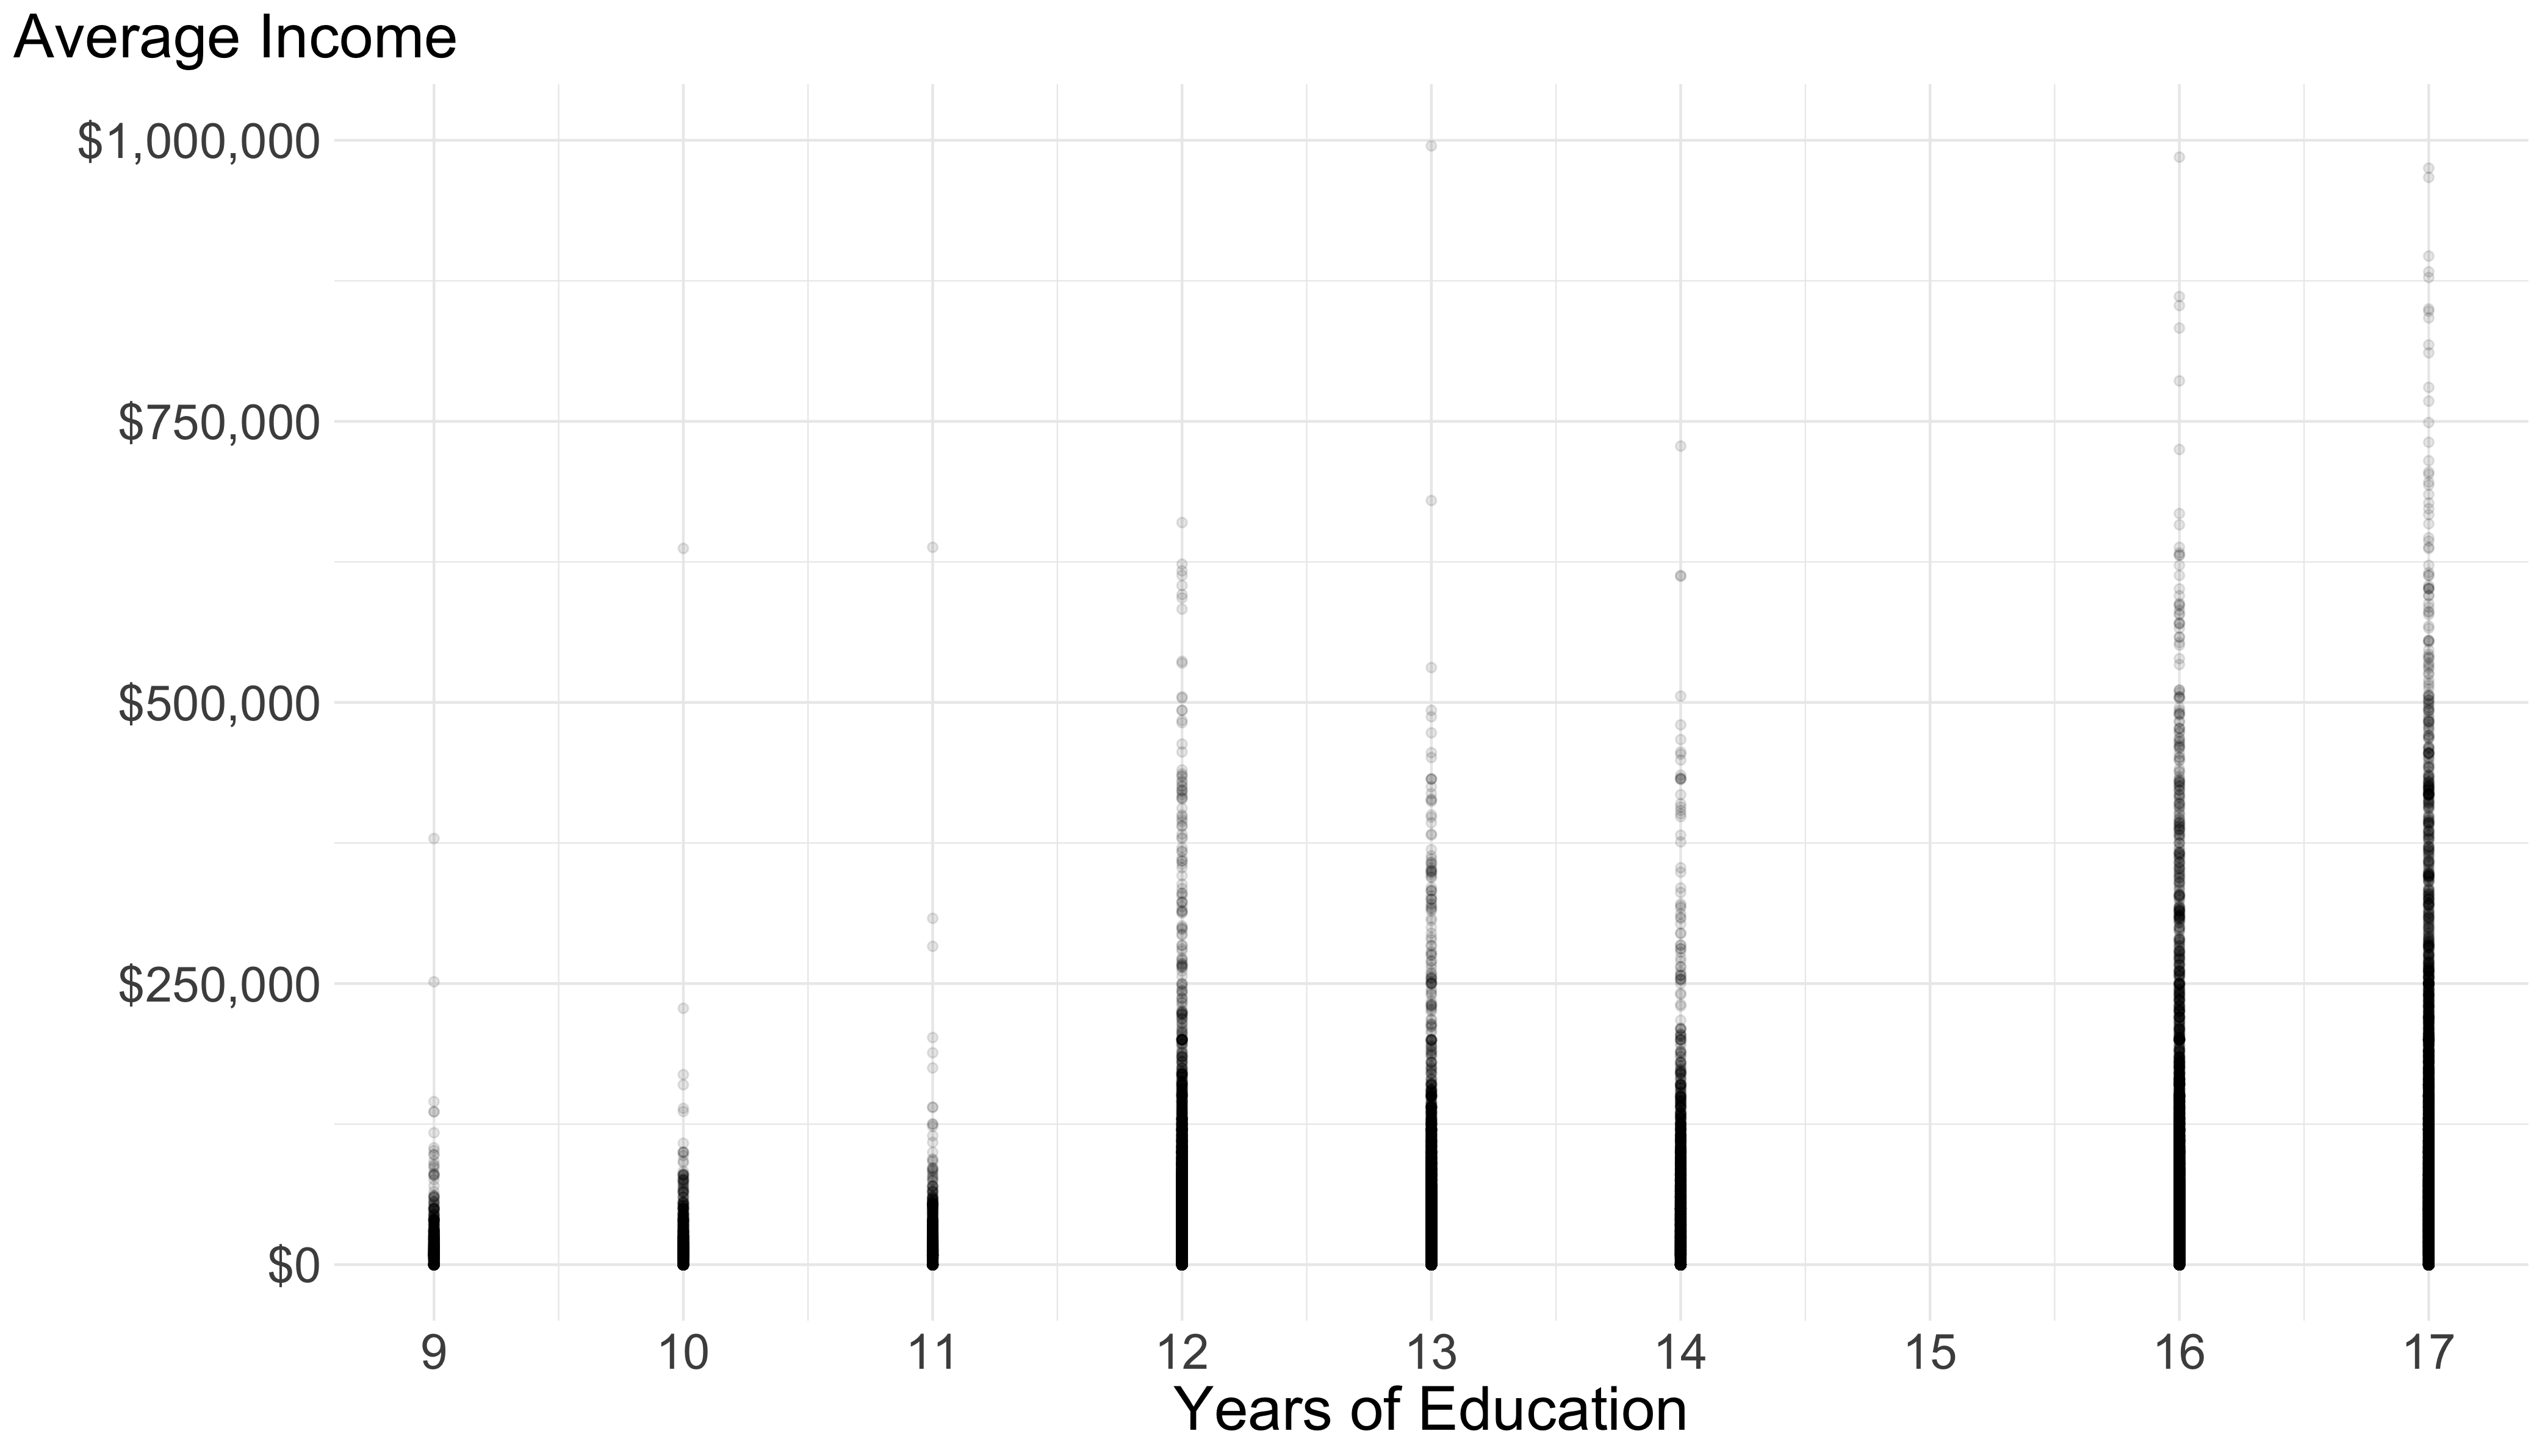
\includegraphics[width=\linewidth]{avg_income_education_scatter.png}
  \end{column}
\end{columns}
\end{frame}

\begin{frame}{Quantile regression}
  \begin{columns}[T] % align columns
    \begin{column}{.3\textwidth}
  \begin{wideitemize}
    \item Education + Income  gradient
    \item Clear heteroskedasticity
    \item Very wide variance, especially at high education
  \end{wideitemize}
  \end{column}%
  \hfill%
  \begin{column}{.7\textwidth}
    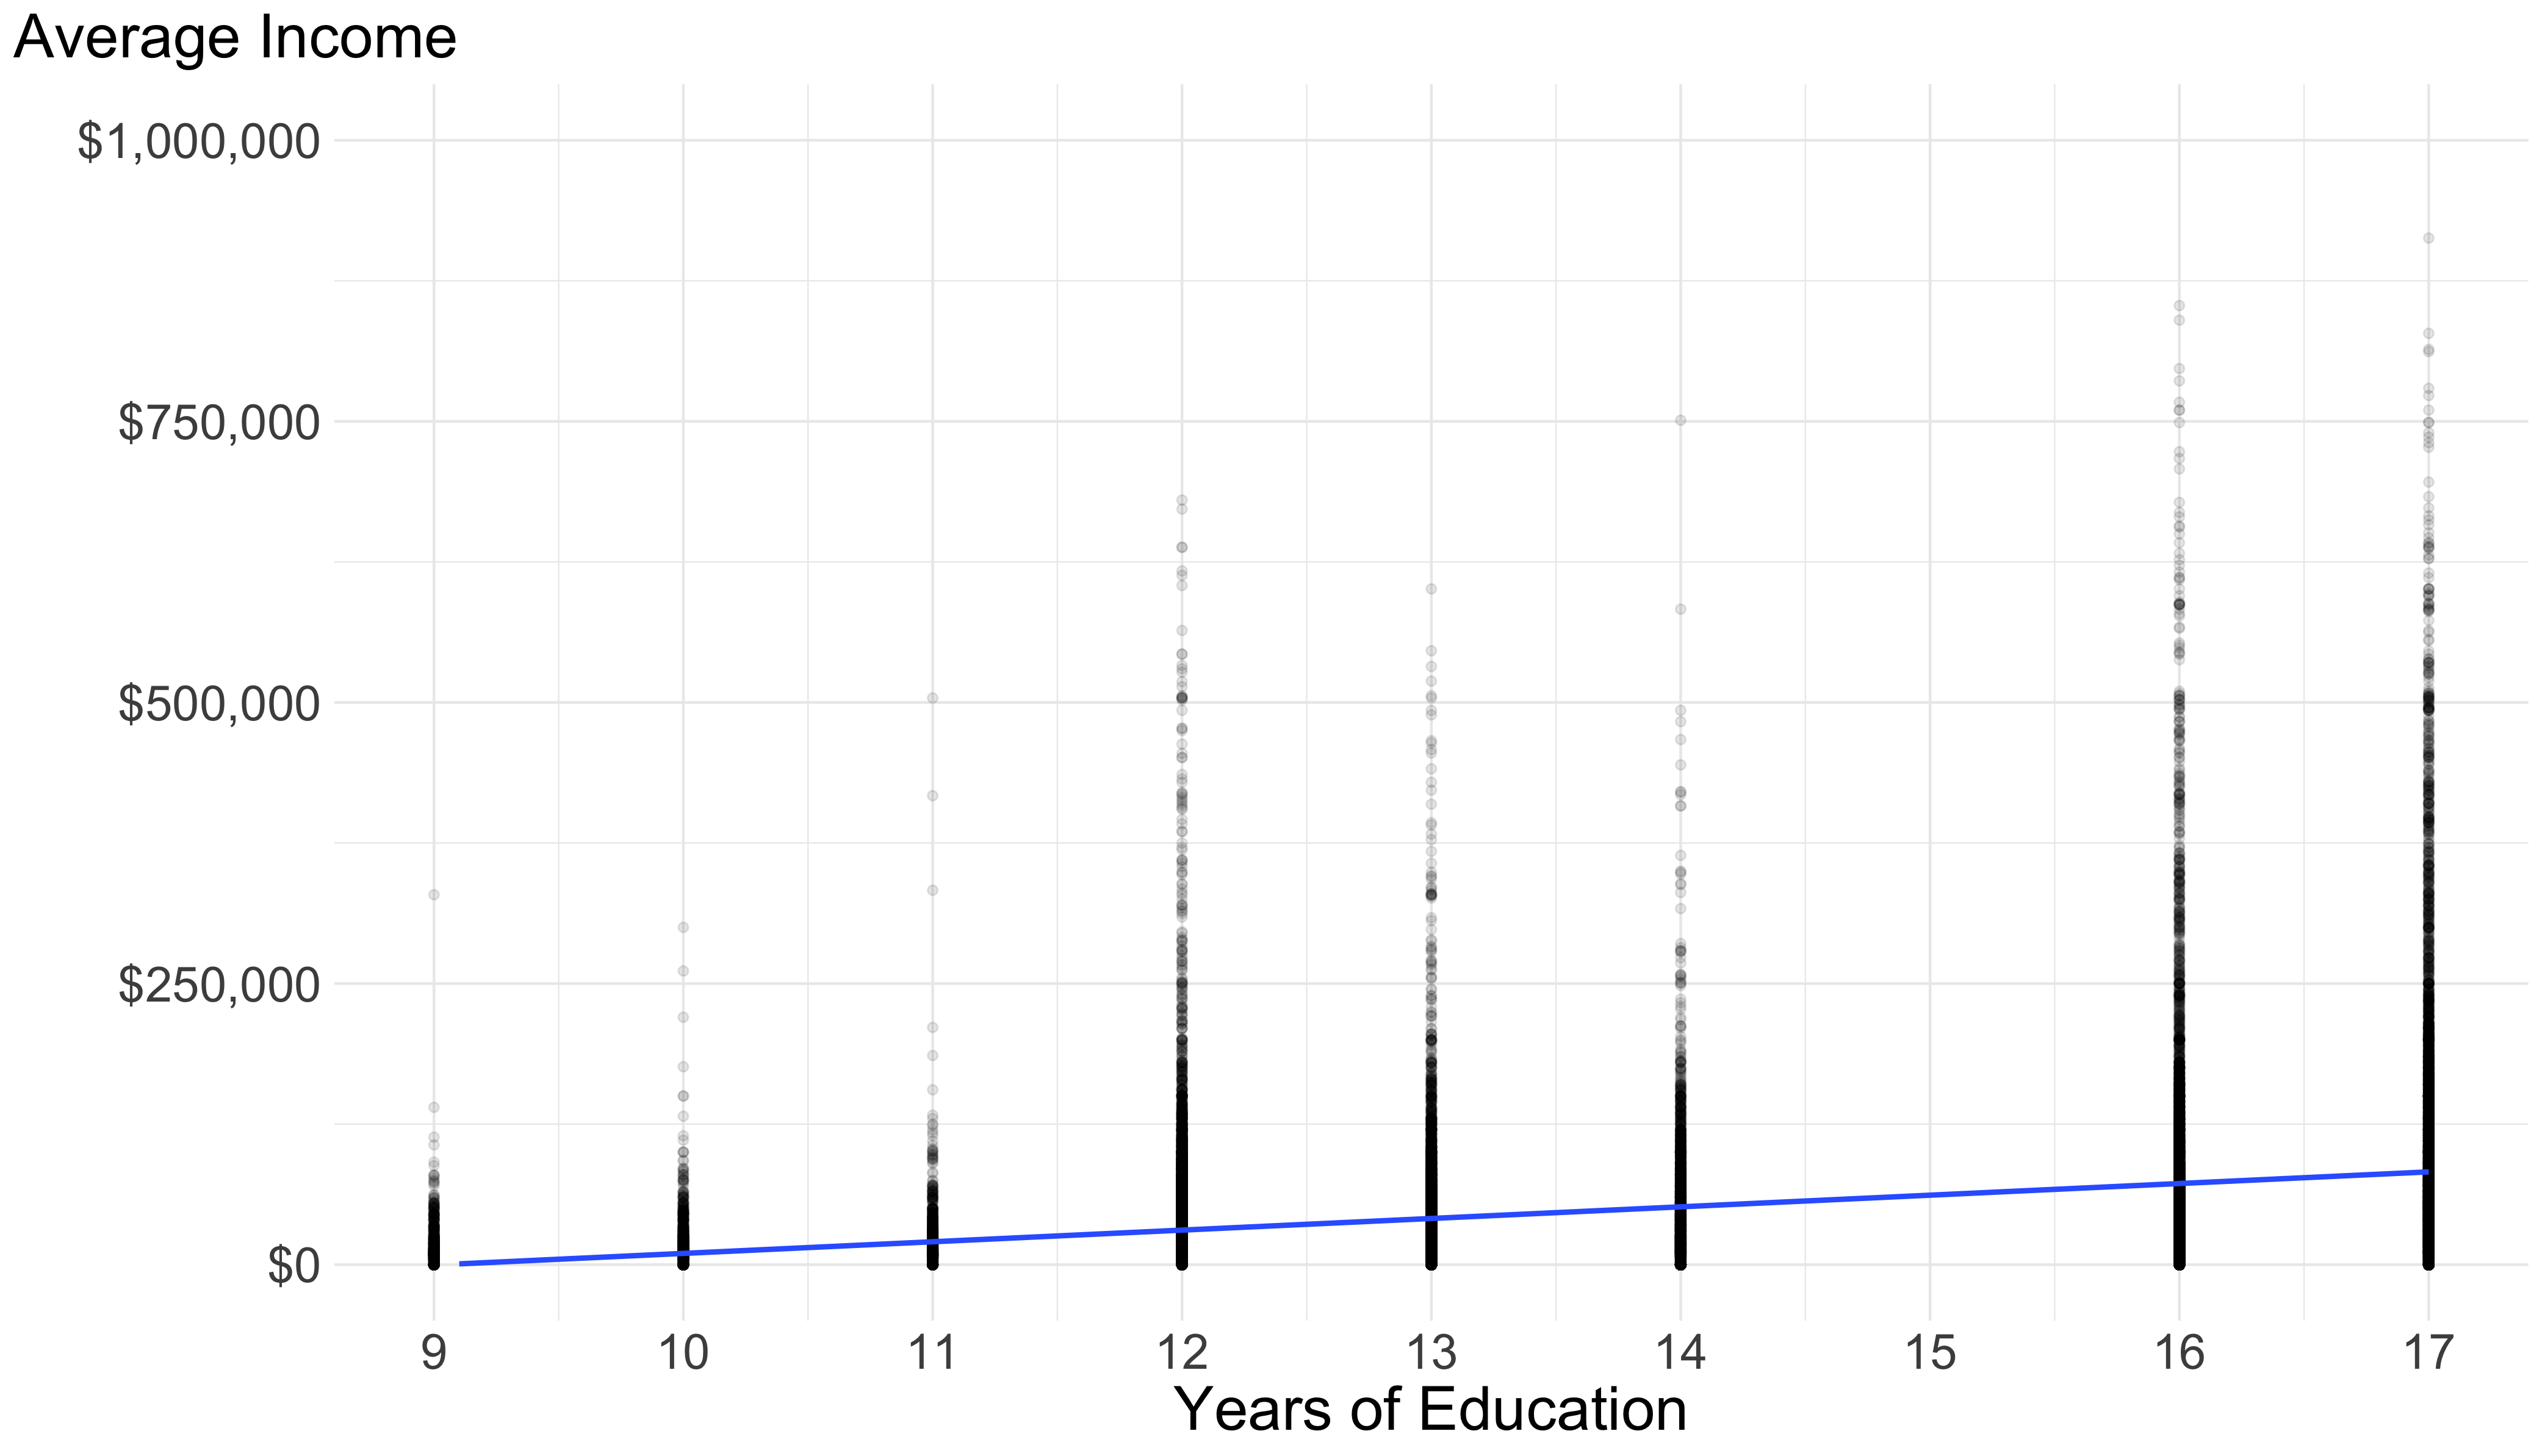
\includegraphics[width=\linewidth]{avg_income_education_scatter_ols.png}
  \end{column}
\end{columns}
\end{frame}
\begin{frame}{Quantile regression}
  \begin{columns}[T] % align columns
    \begin{column}{.3\textwidth}
  \begin{wideitemize}
    \item Education + Income  gradient
    \item Clear heteroskedasticity
    \item Very wide variance, especially at high education
    \item OLS is heaviliy influenced by the tails of income
  \end{wideitemize}
  \end{column}%
  \hfill%
  \begin{column}{.7\textwidth}
    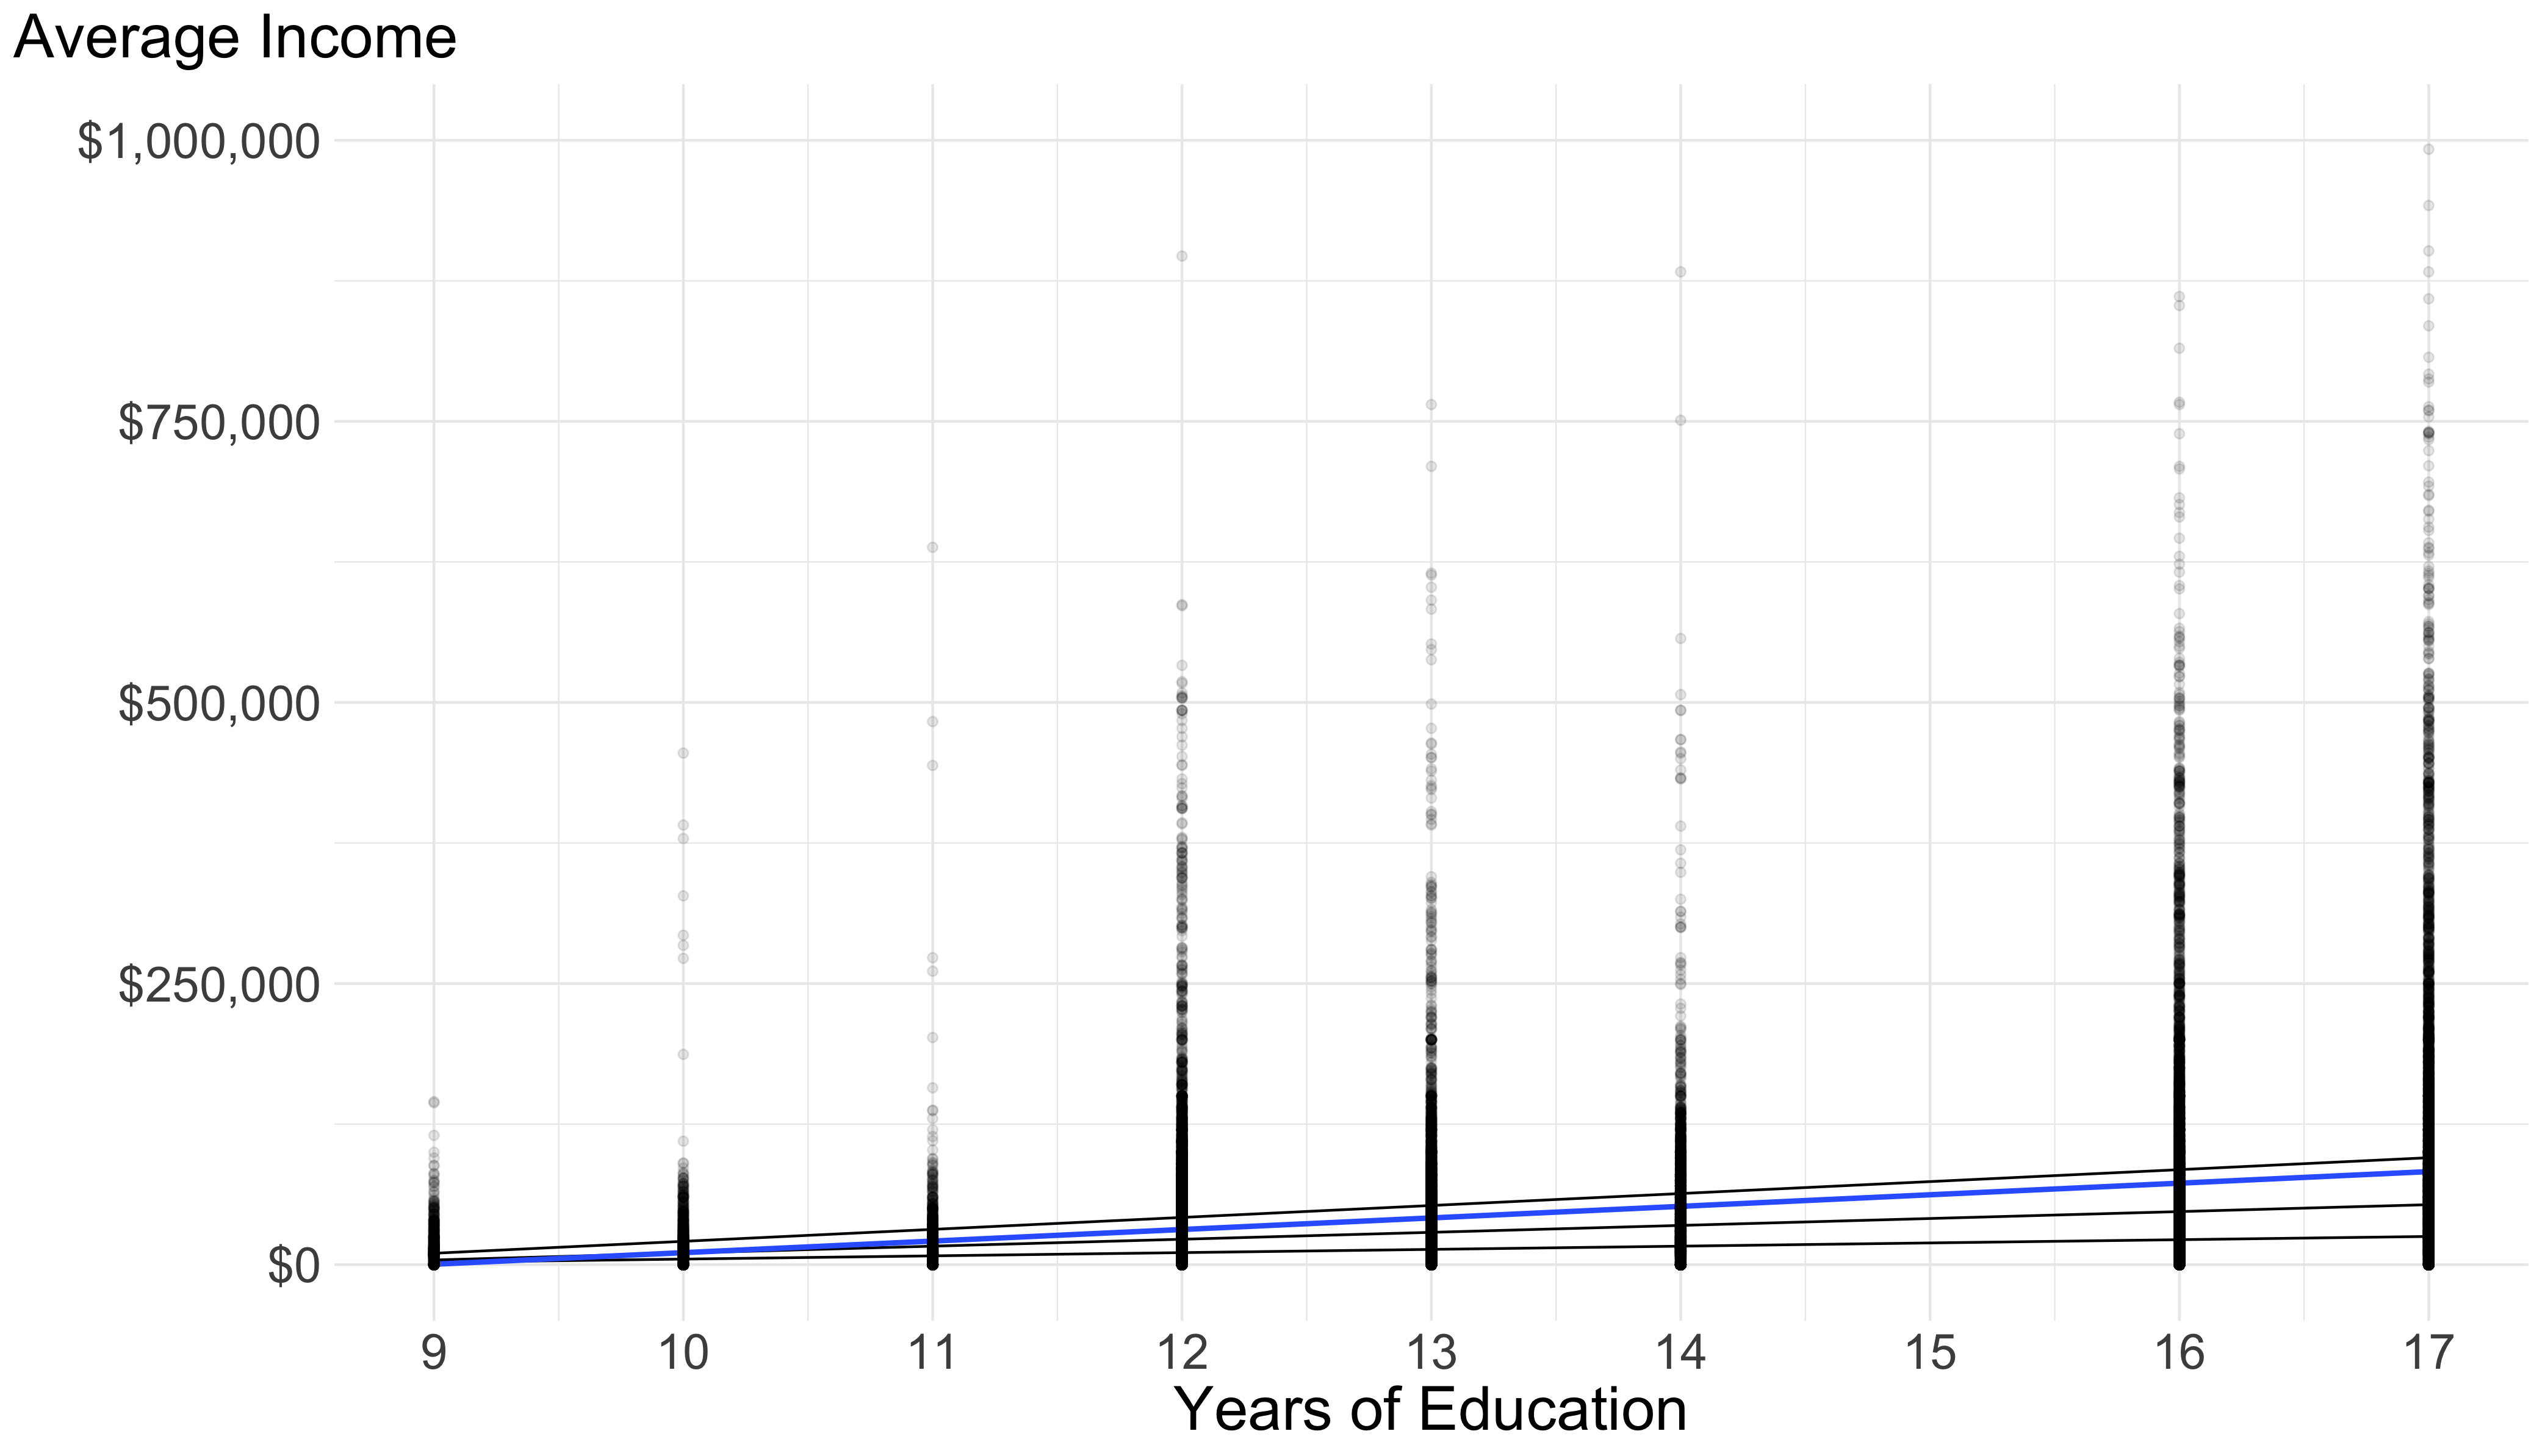
\includegraphics[width=\linewidth]{avg_income_education_scatter_ols_quantile.png}
  \end{column}
\end{columns}
\end{frame}

\begin{frame}{Quantile regression}
  \begin{columns}[T] % align columns
    \begin{column}{.3\textwidth}
  \begin{wideitemize}
    \item Education + Income  gradient
    \item Clear heteroskedasticity
    \item Very wide variance, especially at high education
    \item OLS is heaviliy influenced by the tails of income      
  \end{wideitemize}
  \end{column}%
  \hfill%
  \begin{column}{.7\textwidth}
    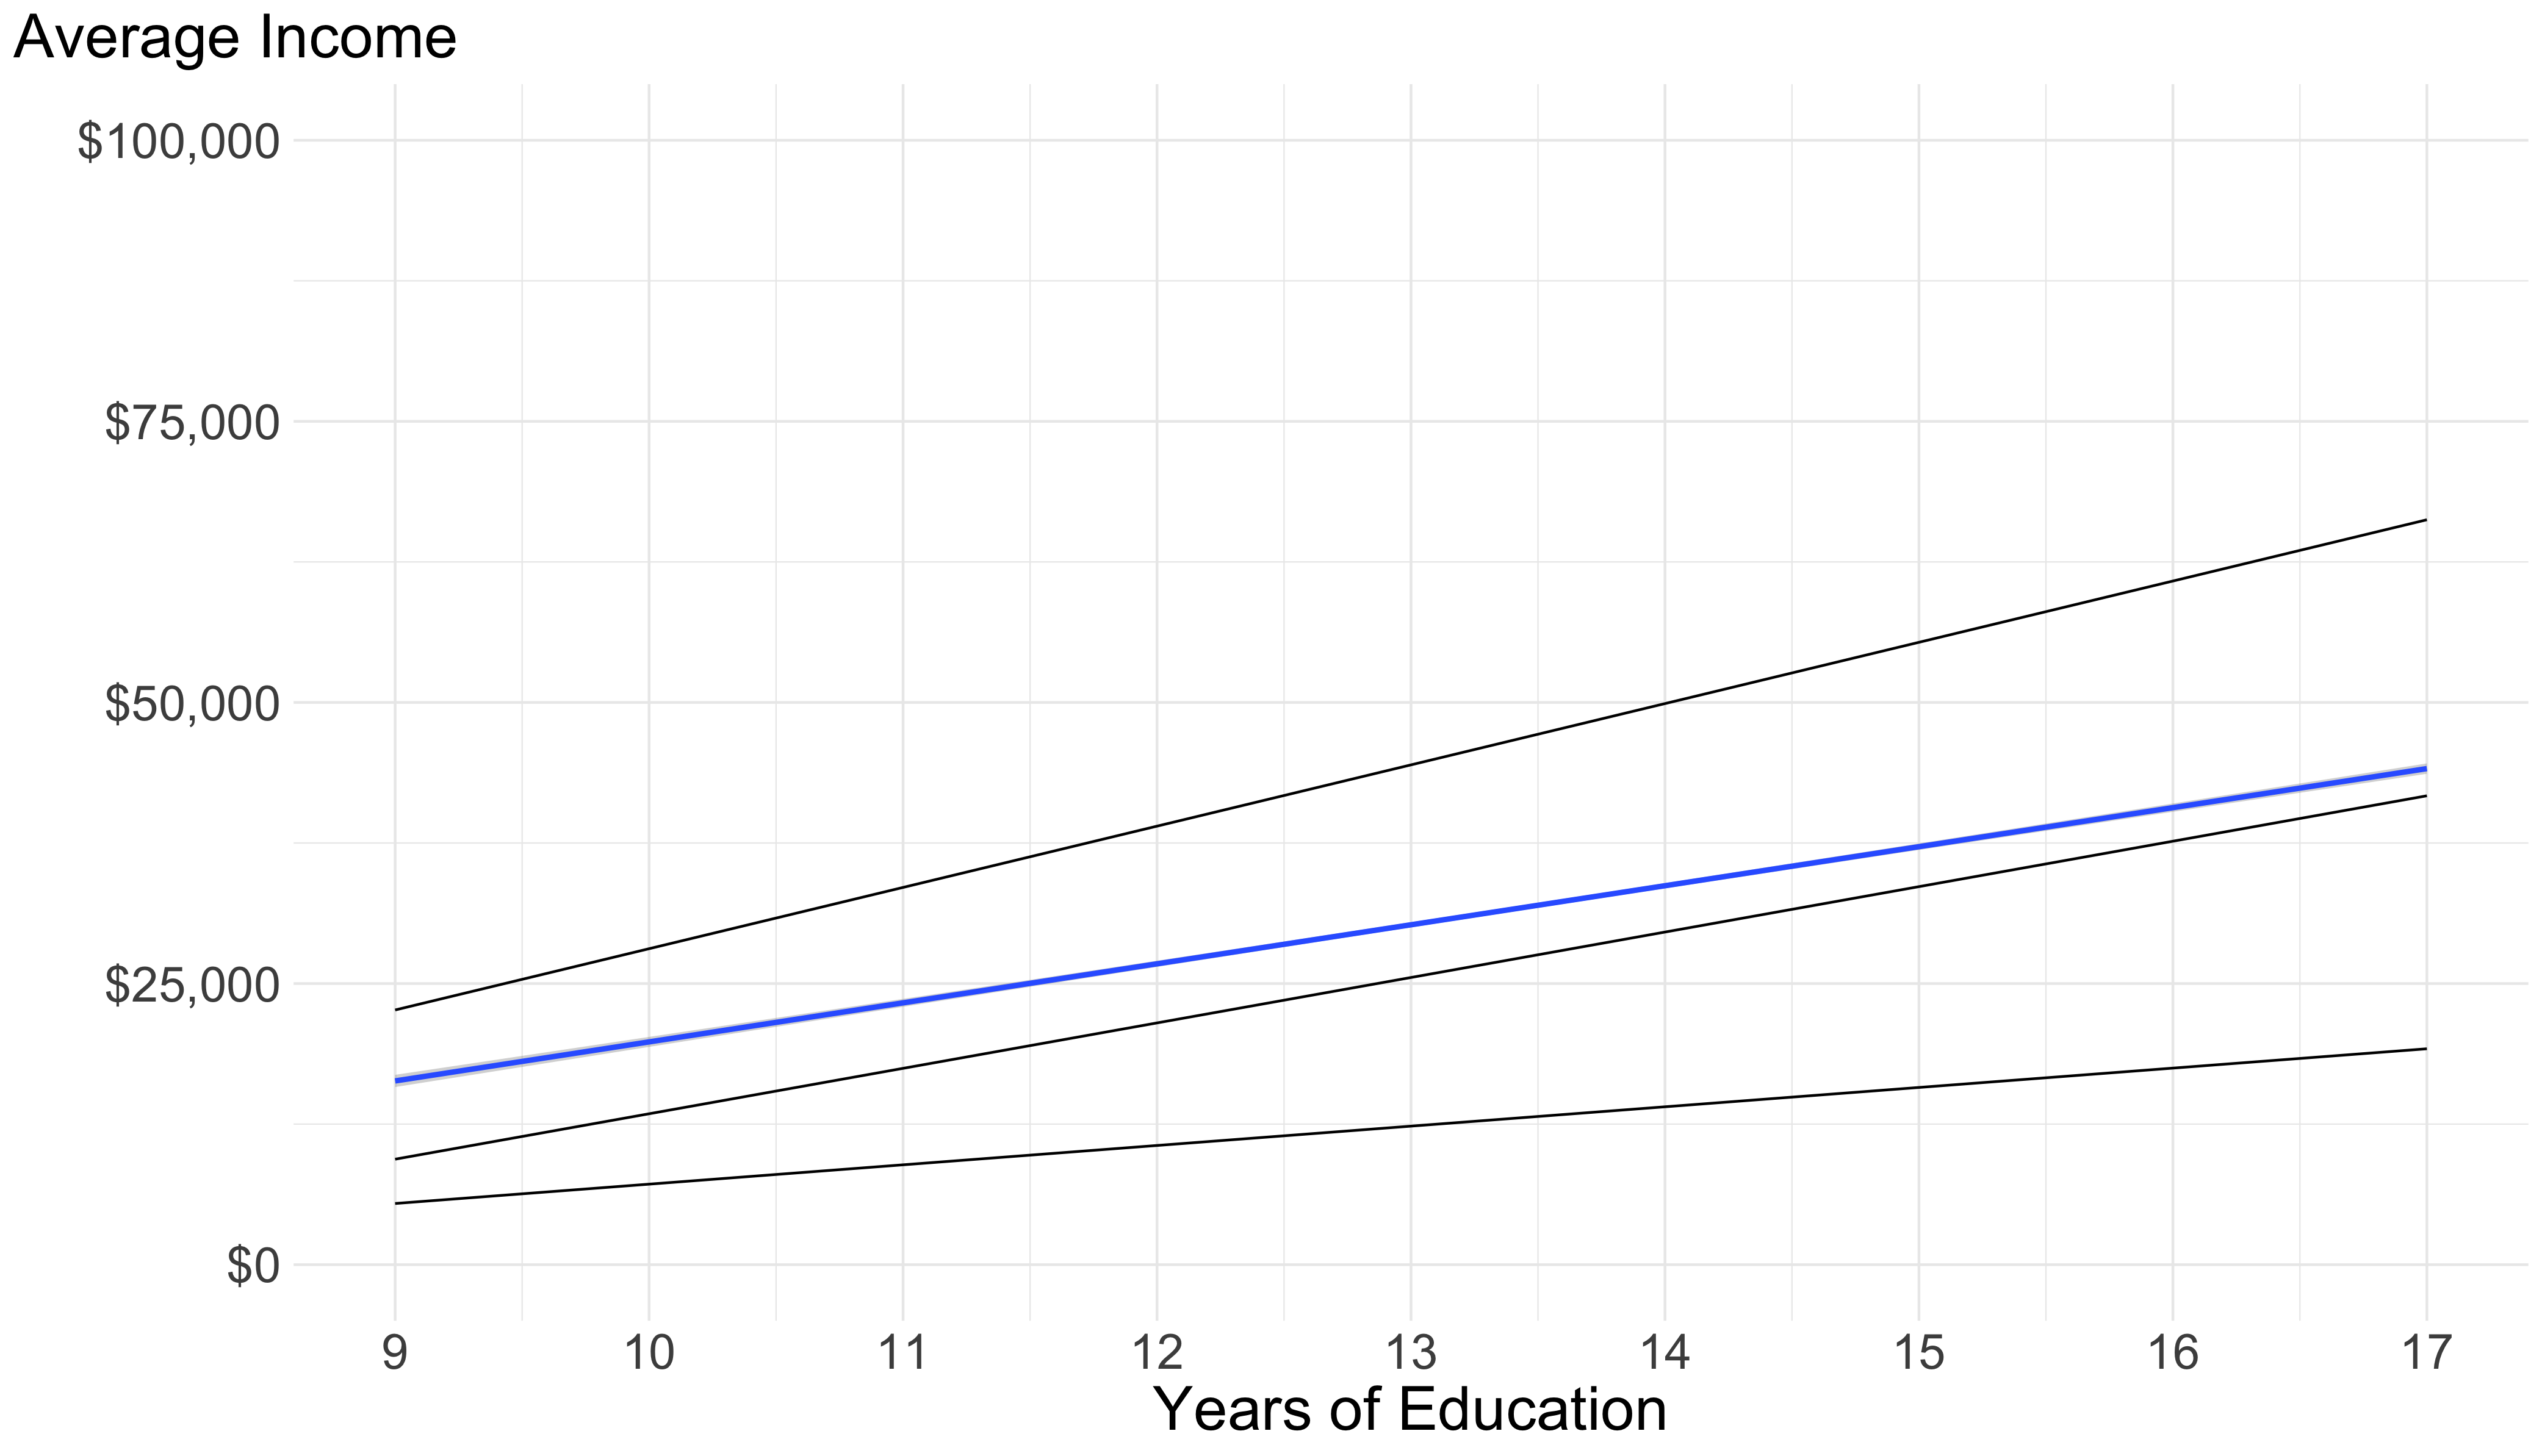
\includegraphics[width=\linewidth]{avg_income_education_scatter_ols_quantile_zoom.png}
  \end{column}
\end{columns}
\end{frame}


\begin{frame}{Interpreting Quantile Coefficients}
  \begin{wideitemize}
  \item   There are some very nice features of this setup.
    \begin{itemize}
    \item Very robust
    \end{itemize}
  \item However, interpreting these coefficients from a structural
    model standpoint is challenging
    \begin{itemize}
    \item Even Koenker's book punts on this issue -- instead pointing
      out that the OLS interpretions are probably wrong!
    \end{itemize}
  \item Why is it so hard? Let's dig into this.
  \end{wideitemize}
\end{frame}

\begin{frame}{Interpreting Quantile Regressions}
  \begin{columns}[T] % align columns
\begin{column}{.6\textwidth}
  \begin{wideitemize}
  \item Consider a binary treatment variable $D_{i}$ -- in fact, let's use the
    NSW program from Lalonde
  \item Consider the very simple OLS verison testing this model using
    the experimental data:
    $$y_{i} = \alpha + D_{i}\beta + \epsilon_{i}$$
  \item Recall that this will estimate our ATE for the treatment
  \item What is the interpretation of this affect?
    \begin{itemize}
    \item $E(Y_{i}(1)) - E(Y_{i}(0))$ -- in other words, the expected
      change in the outcome for a person moving from untreated to
      treated
    \item That's a useful metric!
    \end{itemize}
  \end{wideitemize}
  \end{column}%
  \hfill%
  \begin{column}{.4\textwidth}
    \begin{tabular}{lrr}
      Estimate & Point Est. & SE \\
      \midrule
      $\beta_{OLS}$ &  1794.3  & (632.9)\\
      \end{tabular}
  \end{column}
\end{columns}
\end{frame}

\begin{frame}{Interpreting Quantile Regressions}
  \begin{columns}[T] % align columns
    \begin{column}{.5\textwidth}
      \begin{wideitemize}
      \item Now consider if I did quantile regression instead? What is
        that doing?
      \item Previously, we were comparing means of the two
        distribiutions -- e.g. $Y(1)$ and $Y(0)$.  We did not need to
        specify anything about the joint distribution of $Y(1),Y(0)$
      \item Why does this matter?
        \begin{itemize}
        \item Consider a person sitting in the control group at the 75
          percentile e.g. $Y_{0.75}(0)$
        \item What is their relevant treatment effect?
        \end{itemize}
      \end{wideitemize}
    \end{column}%
    \hfill%
    \begin{column}{.5\textwidth}
      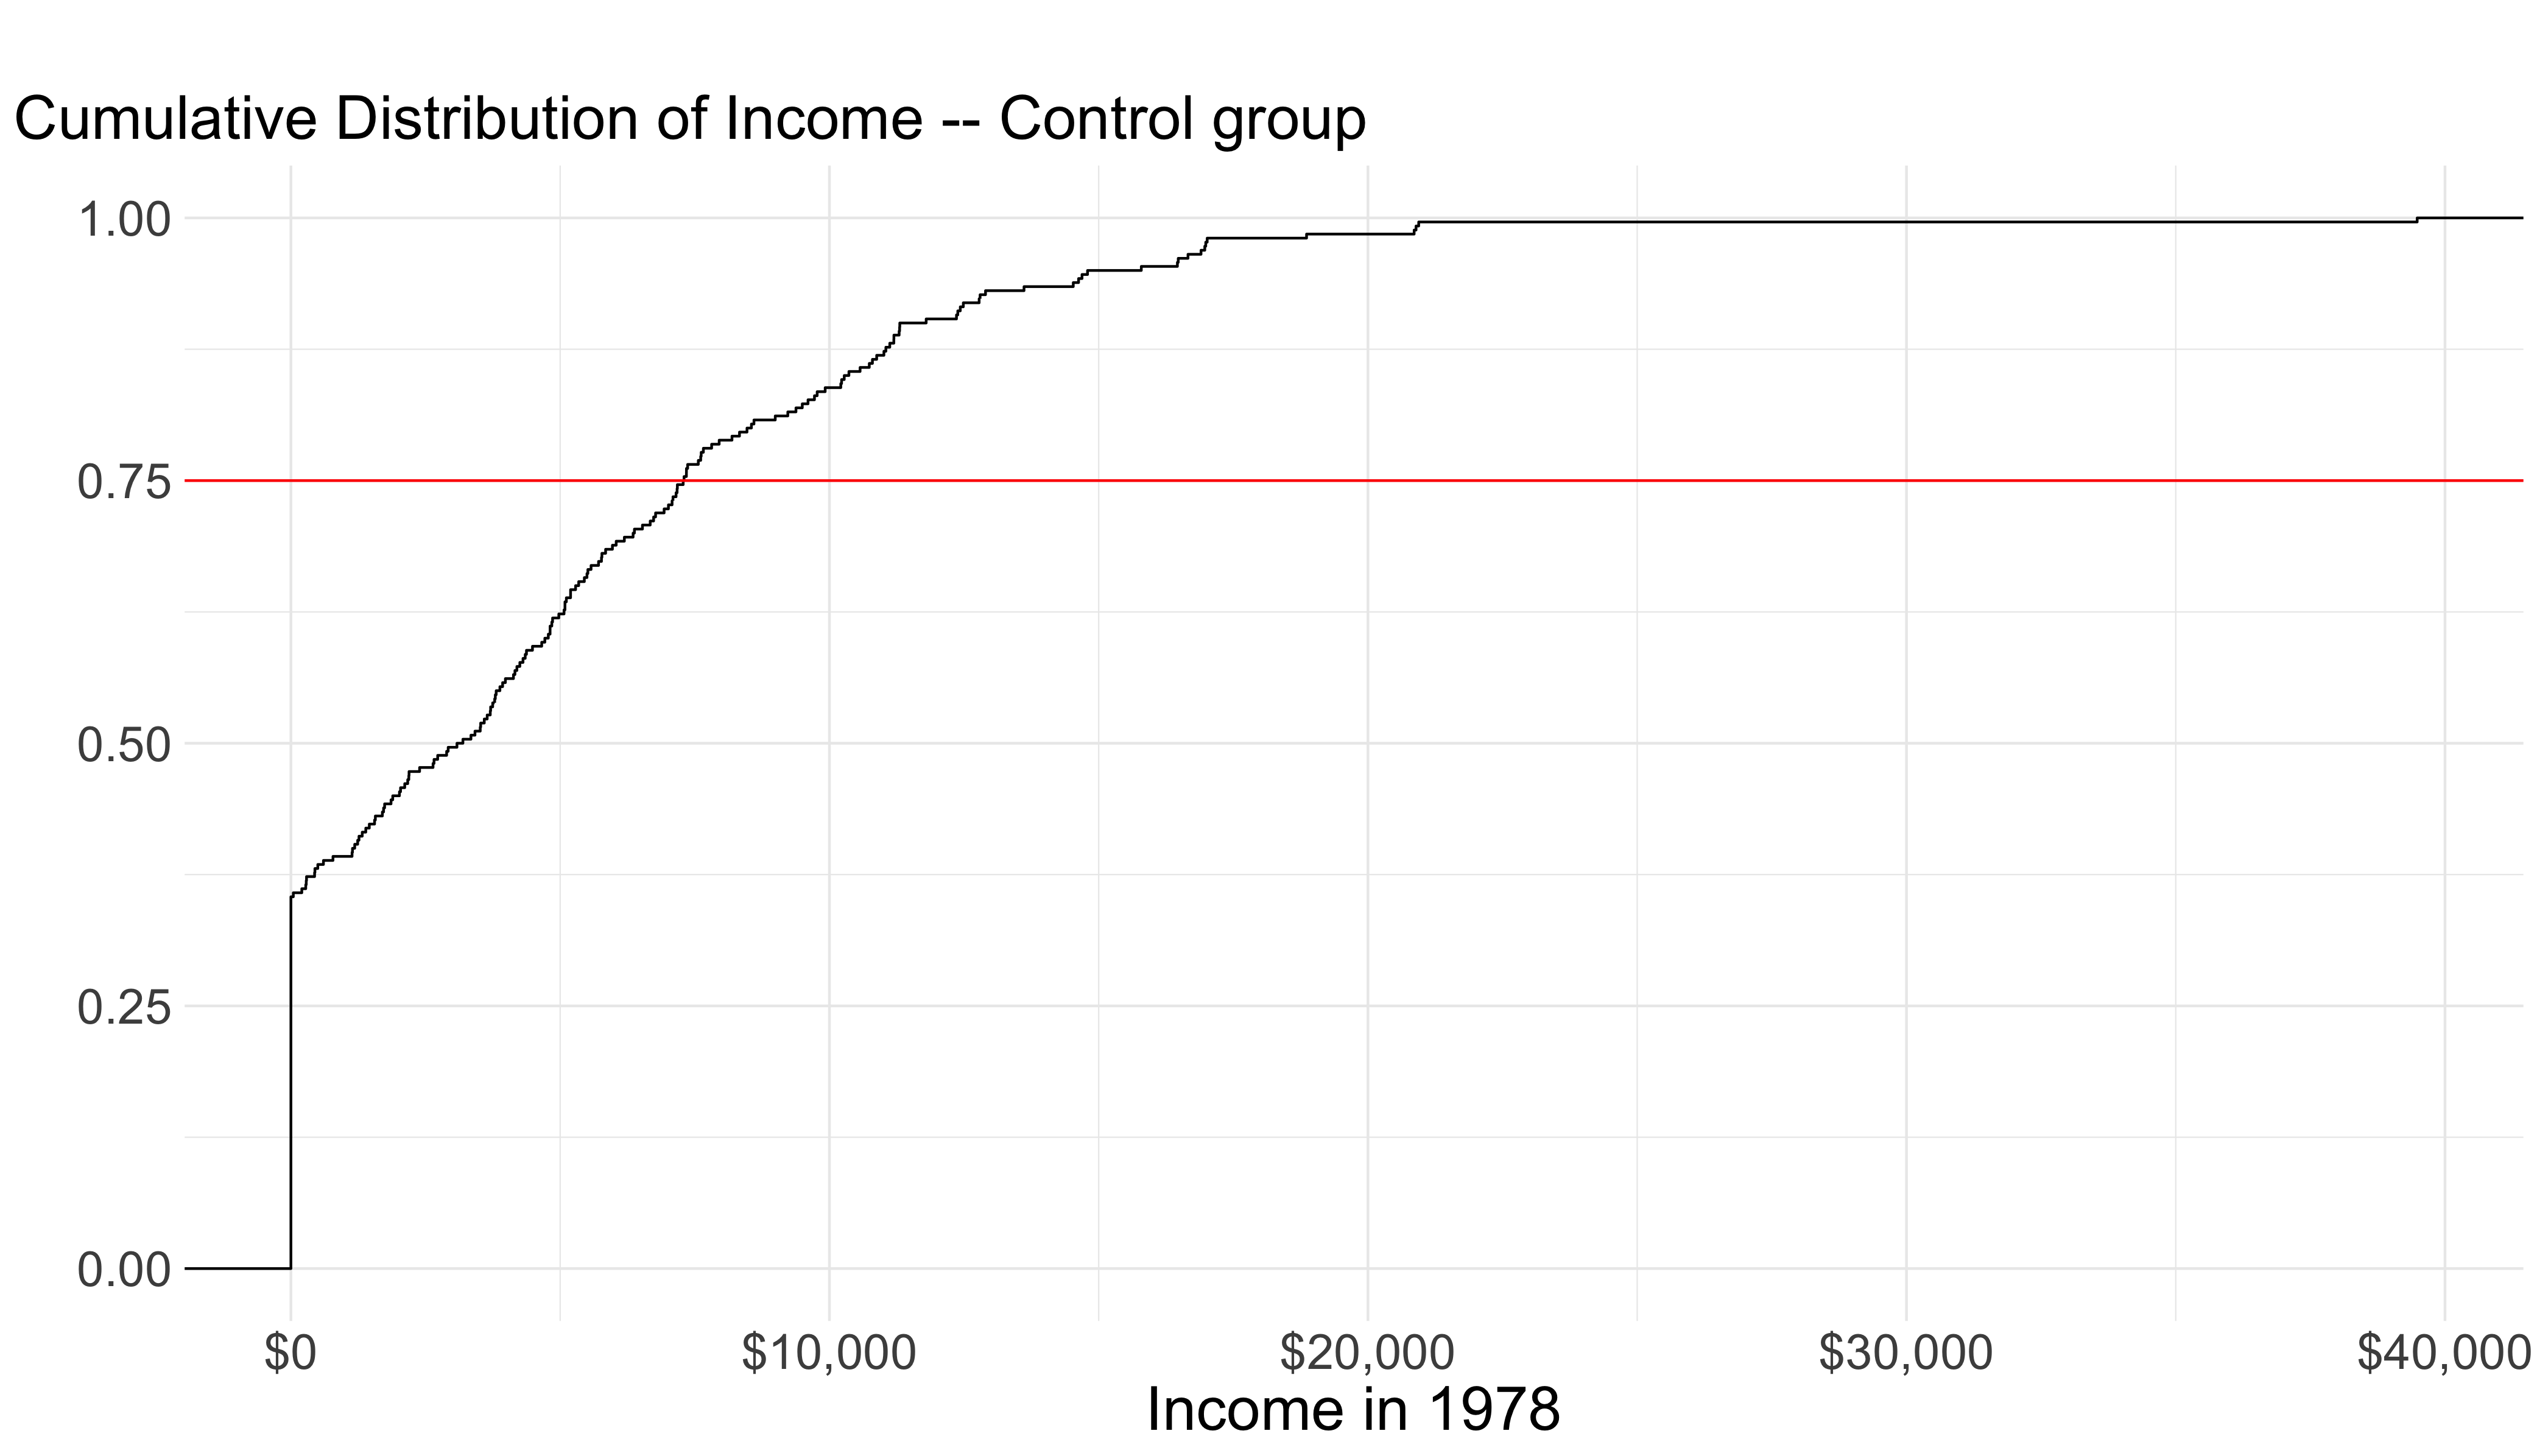
\includegraphics[width=\linewidth]{quantile_cdf_nsw_control75.png}
    \end{column}
  \end{columns}
\end{frame}

\begin{frame}{Interpreting Quantile Regressions}
  \begin{columns}[T] % align columns
    \begin{column}{.7\textwidth}
      \begin{wideitemize}
      \item Types of treatment effects can focus on verisons:
        \begin{enumerate}
        \item Just comparing parts of the \emph{distribution}: $q_{1,\tau} - q_{0,\tau}$ (e.g. Firpo (2005))
        \item Assume rank invariance -- e.g. that individuals' rank
          in the distribiution does not change in moving from
          control to treatment (e.g. Chernozhukov and Hansen (2005))
        \end{enumerate}
      \item The second approach is very strong, and gets you a lot
        of mileage (e.g. extremely useful for IVQR)
      \item The first approach requires weaker assumptions, but then
        we cannot say anything about what the effect of a policy is on
        a person in a given part of the distribiution.
        \begin{itemize}
        \item Instead, our policy takeaways are integrated over changes in the full shape
        \end{itemize}
      \end{wideitemize}
    \end{column}%
    \hfill%
    \begin{column}{.4\textwidth}
    \end{column}
  \end{columns}
\end{frame}

\begin{frame}{Interpreting Quantile Regressions}
  \begin{columns}[T] % align columns
    \begin{column}{.5\textwidth}
      \begin{wideitemize}
      \item Now we can look at the effect of NSW across the distributions
      \item Remarkably homogeneous
      \item 20\% of distributions had zero income, so degenerate
        effects. However, can trace out distributional effects for
        large groups
      \end{wideitemize}
    \end{column}%
    \hfill%
    \begin{column}{.5\textwidth}
      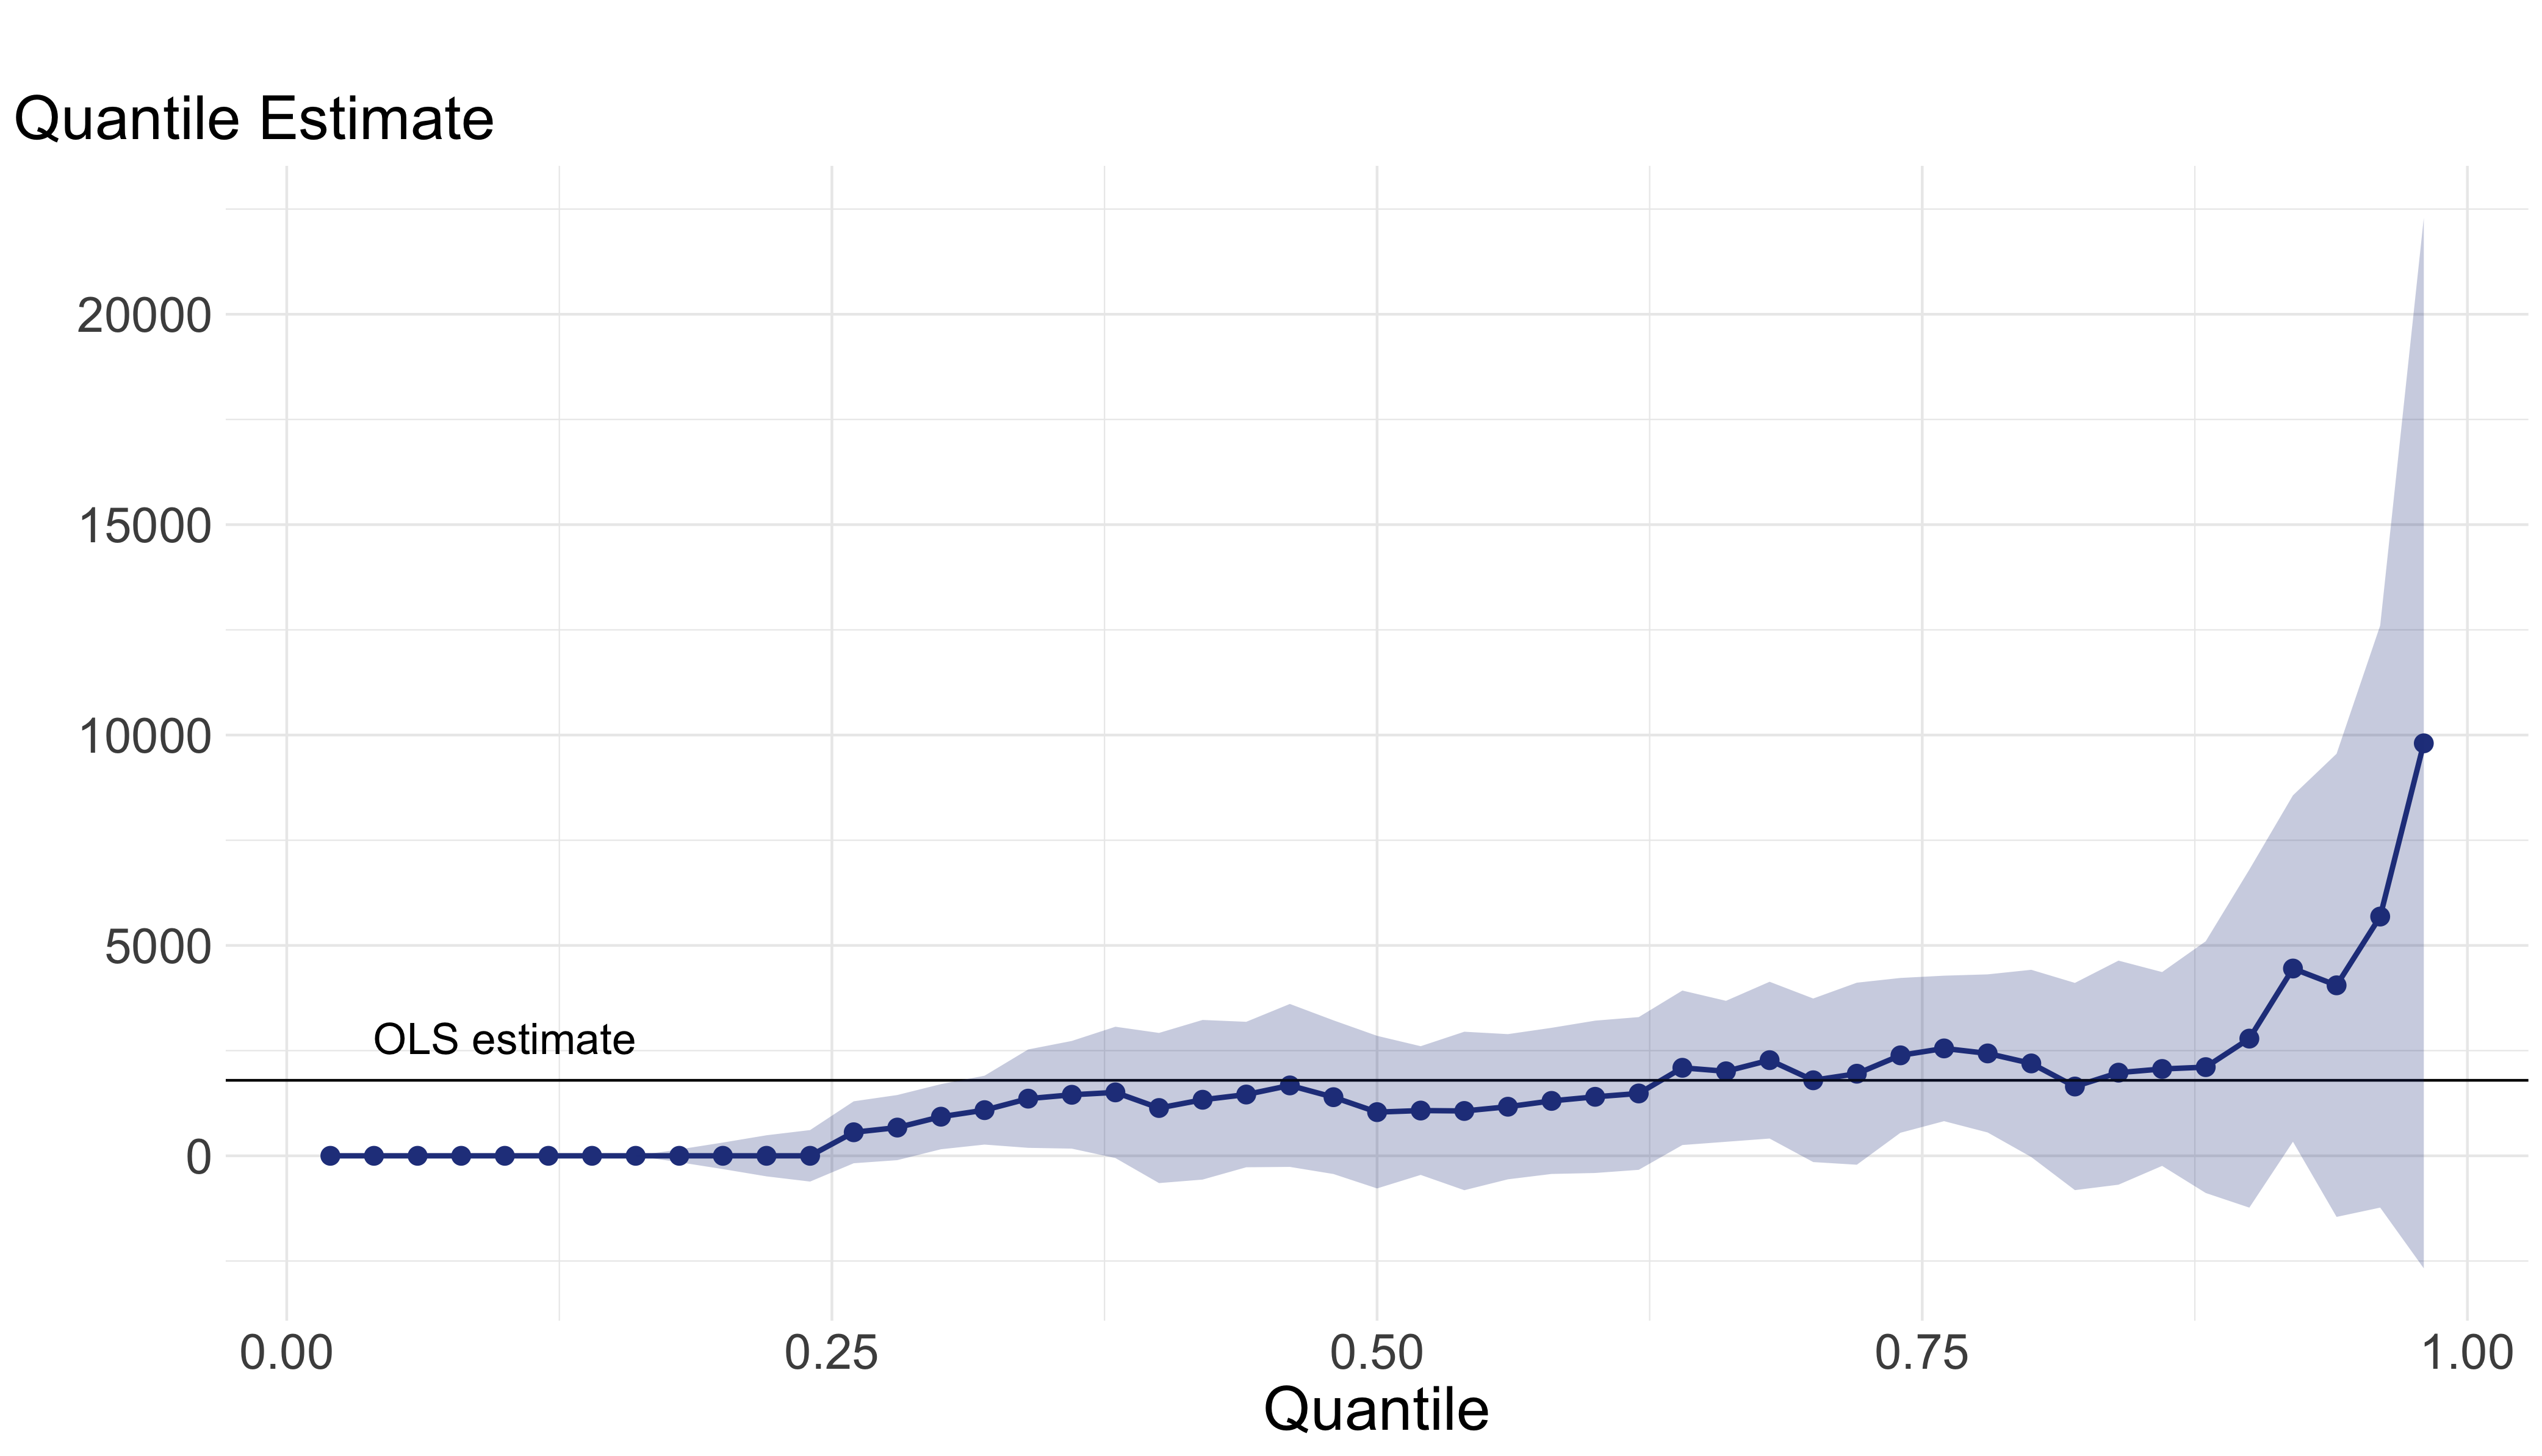
\includegraphics[width=\linewidth]{quantile_plot_nsw.png}
    \end{column}
  \end{columns}
\end{frame}


\begin{frame}{Interpreting Quantile Regressions}
  \begin{columns}[T] % align columns
    \begin{column}{.5\textwidth}
      \begin{wideitemize}
      \item How does this compare efficiency-wise?
      \item Much noisier -- compare median, 75th percentile and 95th
      \item Important to be holistic about estimates in this setting;
        b/c of joint estimation problem of density and quantiles,
        different quantiles can be better estimated
      \end{wideitemize}
    \end{column}%
    \hfill%
    \begin{column}{.5\textwidth}
    \begin{tabular}{lrr}
      Estimate & Point Est. & SE \\
      \midrule
      $\beta_{OLS}$ &  1794.3  & (632.9)\\
      $\beta_{0.5}$ &  1038.3  & (872.3)\\
      $\beta_{0.75}$ & 2342.5  & (893.4)\\
      $\beta_{0.95}$ & 2992.2  & (2973.0)\\
      \end{tabular}
    \end{column}
  \end{columns}
\end{frame}

\begin{frame}{A result from Firpo (2005)}
  \begin{wideitemize}
  \item An analagous IPW estimator which we used for efficient estimation of
    ATE can be used for estimating QTE: $\beta_{\tau} = \hat{q}_{1, \tau} -\hat{q}_{0, \tau}$
    $$\hat{q}_{j, \tau} = \arg\min_{q} \sum_{i=1}^{n}\hat{\omega}_{j,i} \rho_{\tau}(Y_{i} - q), \qquad \hat{\omega}_{1,i} = \frac{T_{i}}{n \hat{p}(X_{i})} \qquad \hat{\omega}_{0,i} = \frac{1-T_{i}}{n (1-\hat{p}(X_{i}))}$$
  \item Indeed, this estimator is the best semiparametric estimator (Firpo (2005))
  \item Note that this follows the same procedure as with the ATE --
    using IPW to identify the quantiles of each underyling distribution
  \end{wideitemize}
\end{frame}

\begin{frame}{Comparing distributions}
        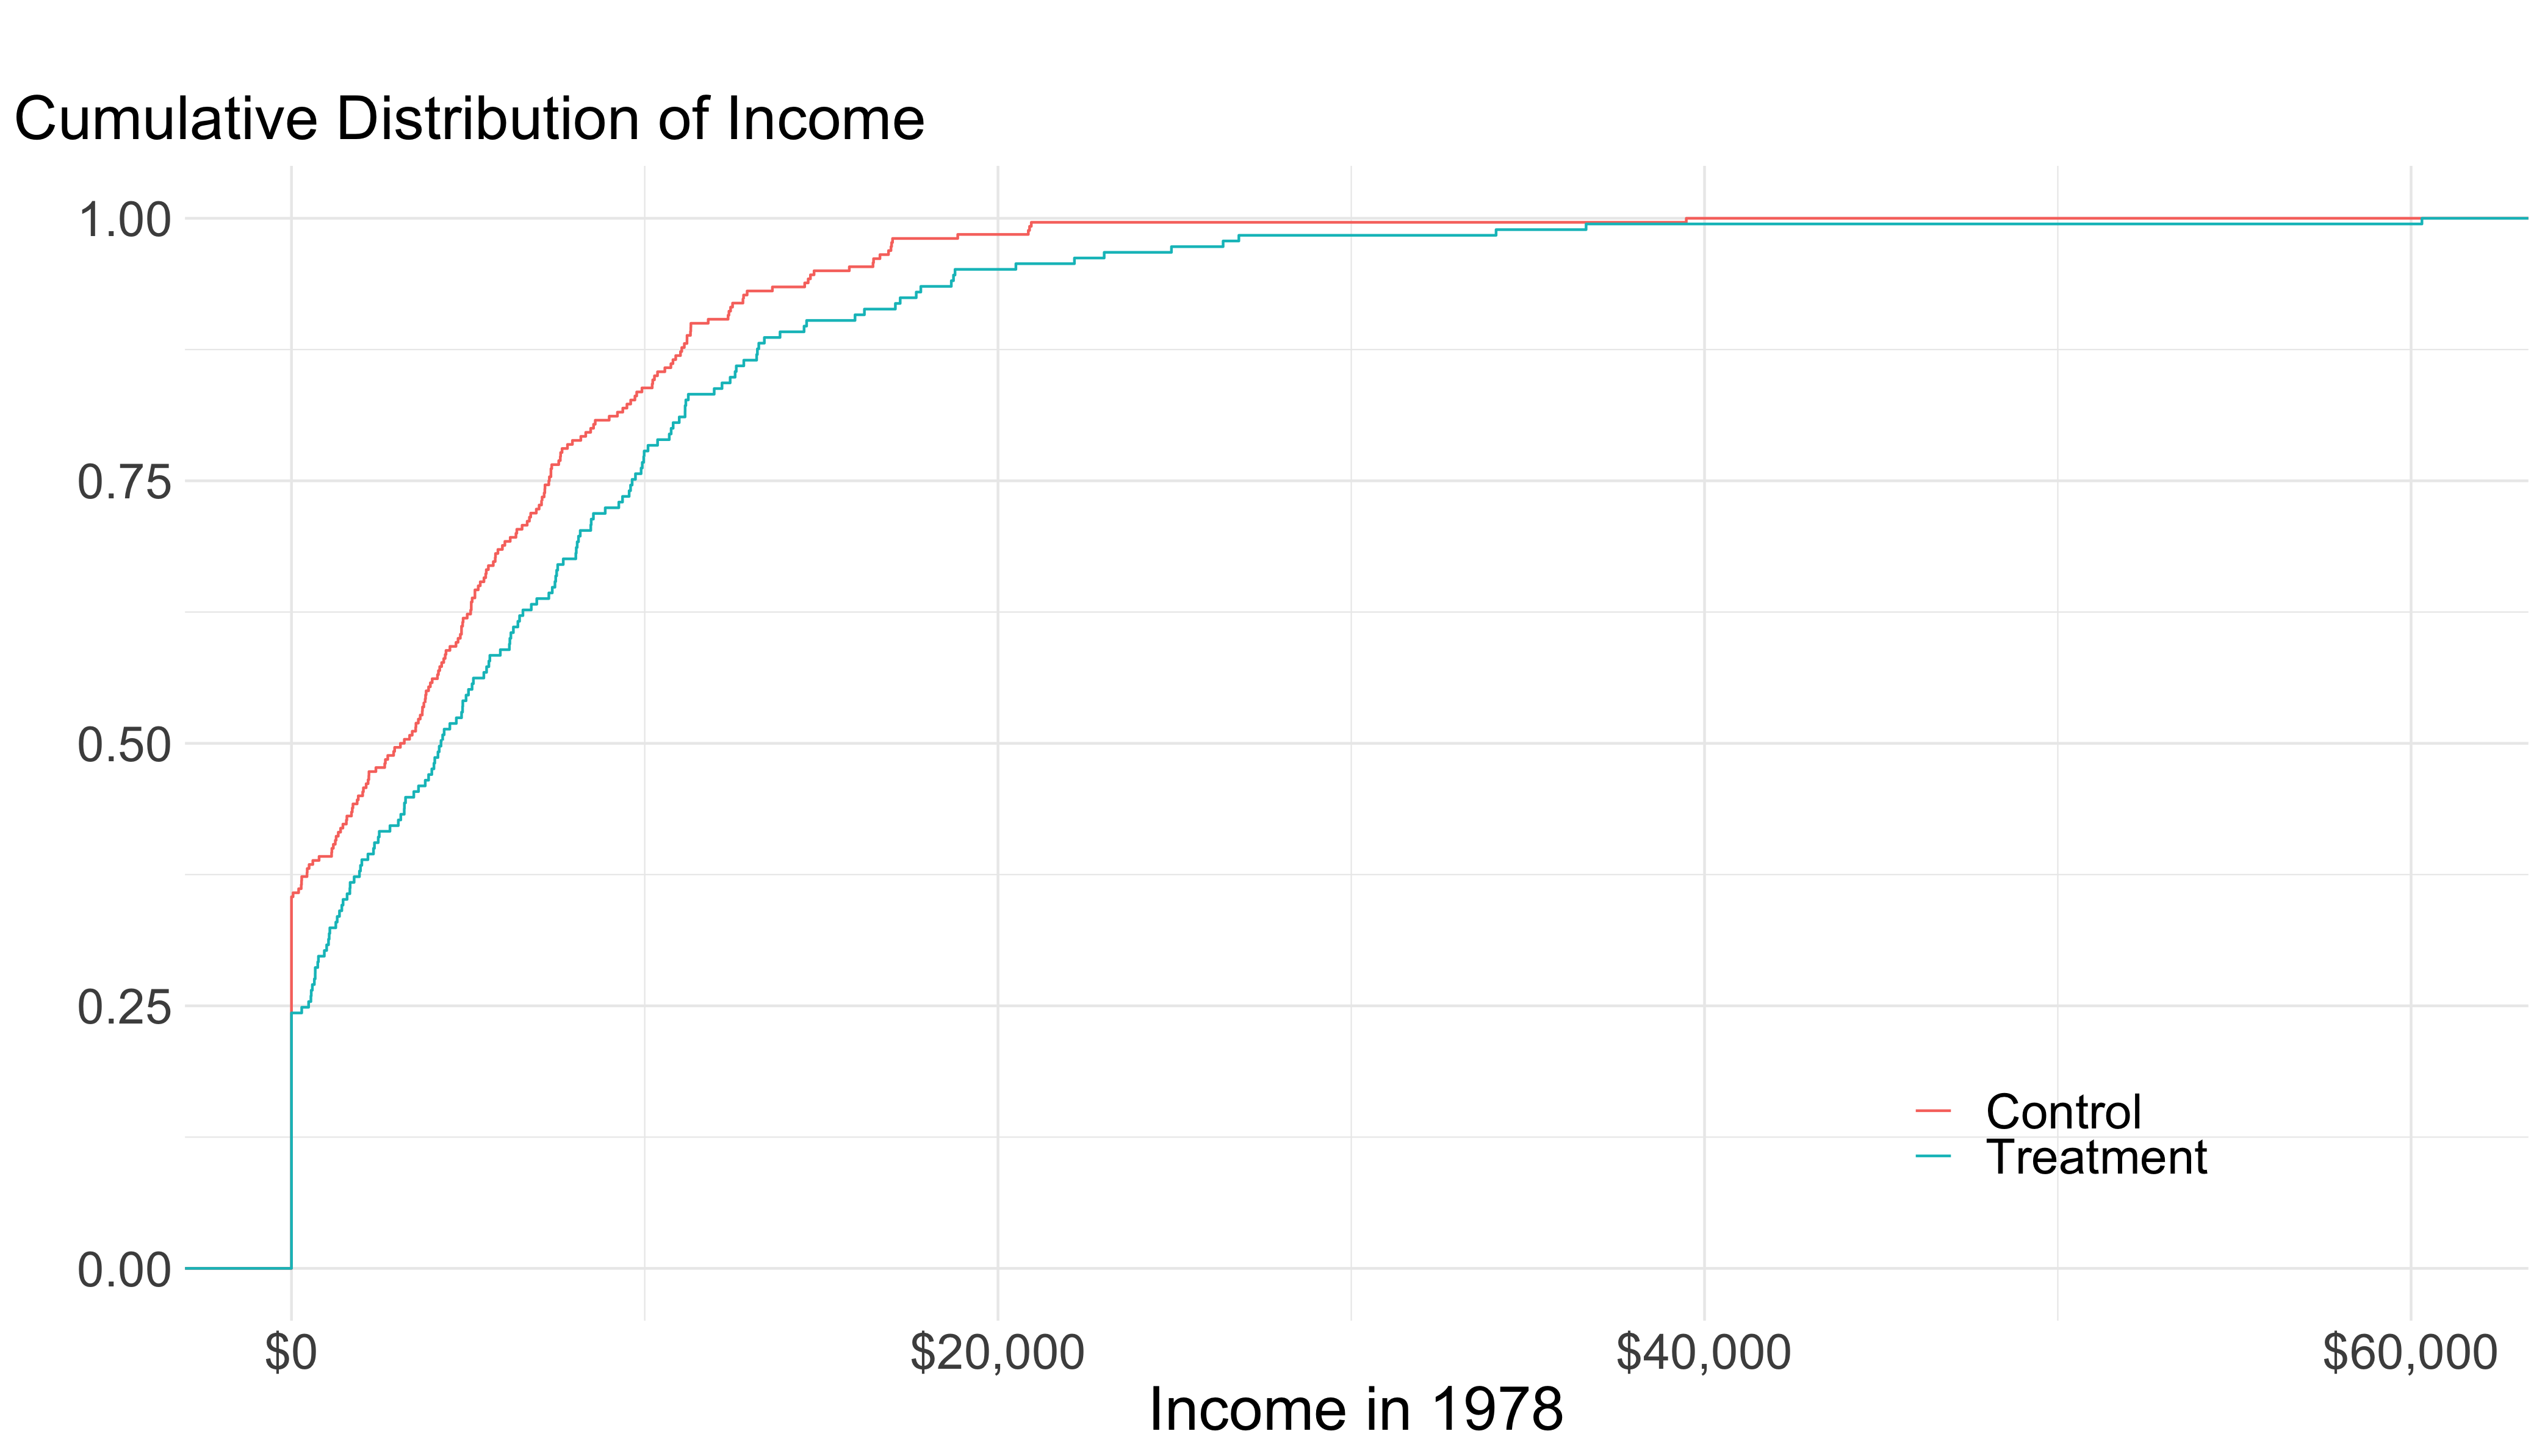
\includegraphics[width=\linewidth]{quantile_cdf_nsw.png}
\end{frame}

\begin{frame}{Last example}
  \begin{wideitemize}
  \item Ok so what? While estimating the range of effects is interesting, it is
    \begin{itemize}
    \item noisier
    \item challenging to interpret in an intuitive way
    \end{itemize}
  \item However, if you have underyling theory that has implications for
    distribiution, quantile regression is the empirical approach for you
  \item A nice paper highlighting this point: Bitler, Gelbach and Hoynes (2006)
  \end{wideitemize}
\end{frame}

\begin{frame}{Bitler, Gelbach and Hoynes (2006)}
  \begin{columns}[T] % align columns
\begin{column}{.5\textwidth}
  \begin{wideitemize}
  \item Comparing the ``Jobs First'' and AFDC programs in CT
  \item Key difference between programs was significantly more
    generous tax treatment in Jobs First (shifting budget line out)
  \item How does implementation of policy affect income?
  \item Implications:
    \begin{enumerate}
    \item Very bottom earners will have no effect
    \item Very top is zero or negative
    \item In between, JF should have positive effect
    \end{enumerate}
  \end{wideitemize}
  \end{column}%
  \hfill%
  \begin{column}{.5\textwidth}
    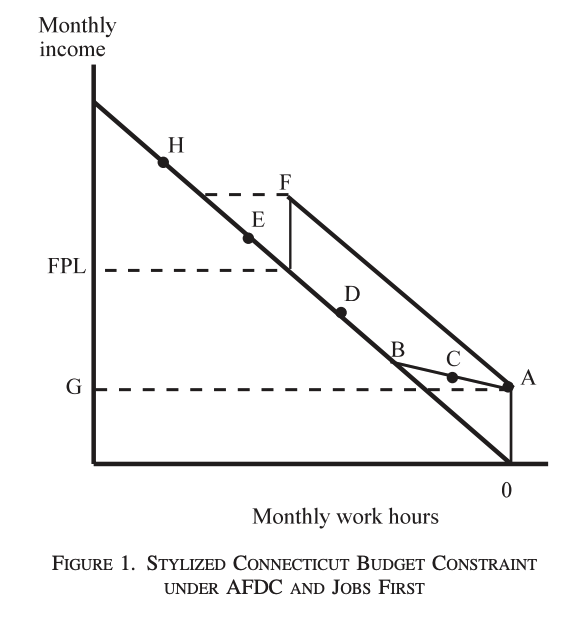
\includegraphics[width=\textwidth]{bitler_budget.png}
  \end{column}
\end{columns}
\end{frame}

\begin{frame}{Bitler, Gelbach and Hoynes (2006) impact on income }
    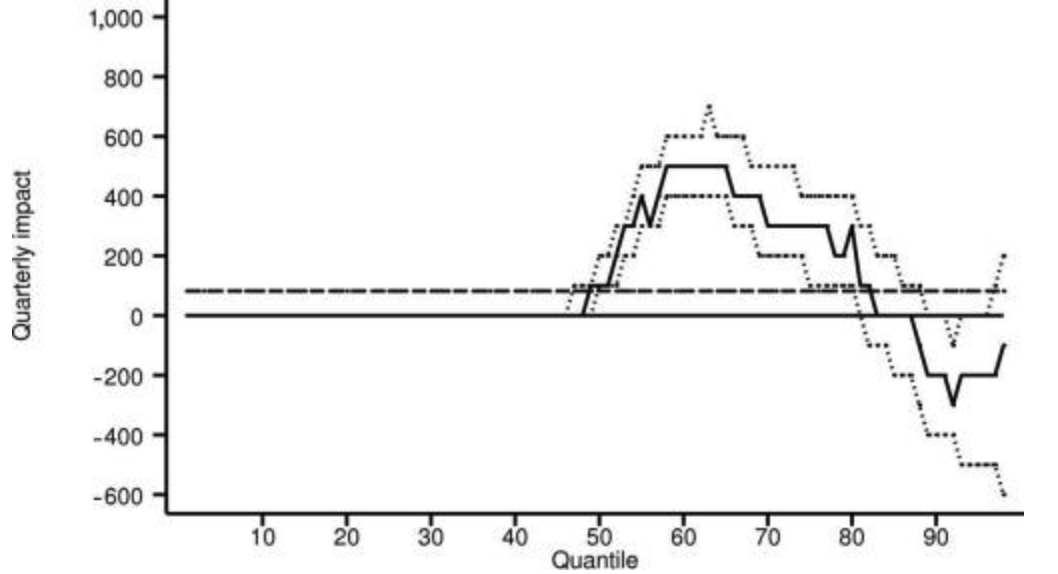
\includegraphics[width=\textwidth]{bitler_QTE.png}
\end{frame}


\begin{frame}{The Upsides of Quantile Regression}
  \begin{wideitemize}
  \item Allows you to characterize the distribution
    \begin{itemize}
    \item  When considering welfare, can be very useful
    \item This can be important for more complicated models
    \item We will revisit when considering hierarchical models
    \end{itemize}
  \item Robust to:
    \begin{itemize}
    \item issues of functional form (e.g. log)
    \item censoring/truncation
    \item outliers
    \end{itemize}
  \item Worth using in your toolkit along with OLS in many applications
    \begin{itemize}
    \item Easy to plug in
    \item \texttt{qreg} in Stata and \texttt{quantreg} in \texttt{R}
    \end{itemize}
  \end{wideitemize}
\end{frame}

\begin{frame}{Issues with Quantile Regression}
  \begin{wideitemize}
  \item Not that fast-- linear programming problem and standard errors
  \item Not additively combinable. E.g., if $Y = Y_{1} + Y_{2}$, not
    possible to decompose and have the effects be comparable.
    \begin{itemize}
    \item This can create issues with fixed effects
    \end{itemize}
  \item Can be challenging to interpet as structural parameters
    \begin{itemize}
    \item Shift focus from parameters to understading how the shape of
      the distribution changes with changes in covariates
    \item Change your estimand!
    \end{itemize}
  \item Standard errors can be wonky -- asymptotic theory is less
    developed, although clustering finally exists! (See Hagemann
    (2017), also Parente and Santos Silva (2016))
  \end{wideitemize}
\end{frame}
\end{document}

